\documentclass[english,xcolor=table]{beamer}
\usepackage{mathptmx}
\usepackage[T1]{fontenc}
\usepackage{color}
\usepackage{babel}
\usepackage{amsmath,amsfonts,amssymb}
\usepackage{ulem}

\usepackage{tikz}
%due to warning \usepackage{pgflibraryshapes}
\usetikzlibrary{shapes} %instead of pgflibraryshapes
\usepackage{xcolor}
\usepackage{fancyvrb,color}
\usepackage{colortbl}
\definecolor{hellgelb}{rgb}{1,1,0.8}
\definecolor{colKeys}{rgb}{0,0,1}
\definecolor{colIdentifier}{rgb}{0,0,0}
\definecolor{colComments}{rgb}{1,0,0}
\definecolor{colString}{rgb}{0,0.5,0}

\definecolor{darkross}{rgb}{0.008,0.412,0.471}
\definecolor{middleross}{rgb}{0.012,0.580,0.663}
\definecolor{lightross}{rgb}{0.016,0.749,0.855}
\definecolor{darkblue}{rgb}{0.067,0.008,0.471}
\definecolor{middleblue}{rgb}{0.094,0.012,0.663}
\definecolor{lightblue}{rgb}{0.122,0.016,0.855}
\definecolor{darkpurple}{rgb}{0.471,0.008,0.412}
\definecolor{middlepurple}{rgb}{0.663,0.012,0.580}
\definecolor{lightpurple}{rgb}{0.855,0.016,0.749}
\definecolor{darkbrown}{rgb}{0.471,0.067,0.008}
\definecolor{middlebrown}{rgb}{0.663,0.094,0.012}
\definecolor{lightbrown}{rgb}{0.855,0.122,0.016}
\definecolor{darkolive}{rgb}{0.412,0.471,0.008}
\definecolor{middleolive}{rgb}{0.580,0.663,0.012}
\definecolor{lightolive}{rgb}{0.749,0.855,0.016}
\definecolor{darkgreen}{rgb}{0.008,0.417,0.067}
\definecolor{middlegreen}{rgb}{0.012,0.663,0.094}
\definecolor{lightgreen}{rgb}{0.016,0.855,0.122}
\definecolor{darkocre}{rgb}{0.471,0.298,0.008}
\definecolor{middleocre}{rgb}{0.663,0.420,0.012}
\definecolor{lightocre}{rgb}{0.855,0.541,0.016}
\definecolor{Gray}{gray}{0.8}	%for highlighting in tables

%http://tex.stackexchange.com/questions/70448/dont-count-backup-slides
\newcommand{\backupbegin}{
   \newcounter{finalframe}
   \setcounter{finalframe}{\value{framenumber}}
}
\newcommand{\backupend}{
   \setcounter{framenumber}{\value{finalframe}}
}

%for \singlespacing
\usepackage{setspace}

%for \ding
\usepackage{pifont}

%\usepackage{caption}
%\usepackage{subcaption}

\usepackage[caption=false,font=footnotesize]{subfig}
%\usepackage{subfigure}

%\renewcommand{\thefootnote}{\arabic{footnote}}
\renewcommand{\footnotesize}{\tiny}

\newcommand\mycolor[2]{\textcolor{#1}{#2}}
\renewcommand{\figurename}{Fig.}

\usepackage{xcolor,tikz,pgflibraryshapes,pgflibraryarrows}
\usetikzlibrary{decorations.text}
\usetikzlibrary{decorations.pathreplacing}


\definecolor{BrightForestGreen}{rgb}{.21,.42,.1}
\definecolor{BloodRed}{rgb}{.86,0,0}

% possible Themes for your beamer-slide-show
%\usetheme{Warsaw}	       %this is super - the section and subsection names dont actually show up on the slides ever, but this theme shows it in the header
% \usetheme{AnnArbor}	    %nice one
%\usetheme{Antibes}		     %
% \usetheme{Bergen}
%\usetheme{Berkeley}		    %nice but looks incomplete :(
%\usetheme{Berlin}				% weird circles in header :(
% \usetheme{Boadilla}		    	% simple, and no header
% \usetheme{boxes}		       %removes all boxes! very simplistic :)
% \usetheme{CambridgeUS}	 		%red headers with section/subsection
%\usetheme{Copenhagen}		%similar to Warsaw!
%\usetheme{Darmstadt}			% weird circles in header :(
% \usetheme{default}
%\usetheme{Dresden}			%% weird circles in header :(
%\usetheme{Frankfurt}
%\usetheme{Ilmenau}
%\usetheme{Goettingen}	  %
%\usetheme{Hannover}	    %
% \usetheme{JuanLesPins}
%\usetheme{Luebeck}		     %
\usetheme{Madrid}				%no section/subsection in headers, blue
%\usetheme{Malmoe}
%\usetheme{Marburg}
%\usetheme{Montpellier}
%\usetheme{PaloAlto}
%\usetheme{Pittsburgh}
%\usetheme{Rochester}			%title bar too broad
%\usetheme{Singapore}
%\usetheme{Szeged}

% color-themes
%\usecolortheme{beaver}
%\usecolortheme{
%       albatross | beaver | beetle |
%       crane | default | dolphin |
%       dove | fly | lily | orchid |
%       rose |seagull | seahorse |
%       sidebartab | structure |
%       whale | wolverine
%}

% customizeable font-themes
%\usefonttheme{
%       default | professionalfonts | serif |
%       structurebold | structureitalicserif |
%       structuresmallcapsserif
%}

% possible inner-theme options
%\useinnertheme{
%       circles | default | inmargin |
%       rectangles | rounded
%}

% possible outer-theme options
%\useoutertheme{
%       default | infolines | miniframes |
%       shadow | sidebar | smoothbars |
%       smoothtree | split | tree
%}
\usepackage[absolute,overlay]{textpos}

\newenvironment<>{varblock}[2][\textwidth]{%
  \setlength{\textwidth}{#1}
  \begin{actionenv}#3%
    \def\insertblocktitle{#2}%
    \par%
    \usebeamertemplate{block begin}}
  {\par%
    \usebeamertemplate{block end}%
  \end{actionenv}}

\makeatletter
\setbeamercovered{transparent}
\beamertemplatetransparentcovereddynamic
\setbeamertemplate{footline}[frame number]
% \newtheorem*{bem}{Bemerkung}

%http://tex.stackexchange.com/questions/46987/centered-frame-title-in-beamer
\setbeamertemplate{frametitle}[default][center]

\makeatother

\begin{document}
% 	\title[Relation-aware Resource Provisioning and Management for Virtualized Services]{Relation-aware Resource Provisioning and Management for Virtualized Services}
	\title{Resource Provisioning and Usage Optimization in Virtualized Environments}
	\author[Sujesha Sudevalayam]{Sujesha Sudevalayam}
	\date[January 13th, 2015]{January 13th, 2015 \\ Pre-synopsis Presentation}
	\institute[IIT Bombay]{Department of Computer Science and Engineering \\ Indian Institute of Technology Bombay \\ \{sujesha\}@cse.iitb.ac.in}

	\subject{Subject}

	%%%%%%%%%%%%% SLIDE %%%%%%%%%%%%%%
	\frame{
		\titlepage
	}

%     %%%%%%%%%%% SLIDE %%%%%%%%%%%%%%
%     \frame{
% 		\frametitle{Talk Outline}
% 	    \tableofcontents
%     }
	
    %%%%%%%%%%%%% SLIDE %%%%%%%%%%%%%%
    \section{Introduction}
      \subsection{Pay-per-Use Service Model}
    \begin{frame}
%       \frametitle{* as a Service}
        \frametitle{Pay-Per-Use Service Model}
         \begin{columns}
            \column{0.33\textwidth}
                \begin{tabular}{c}
                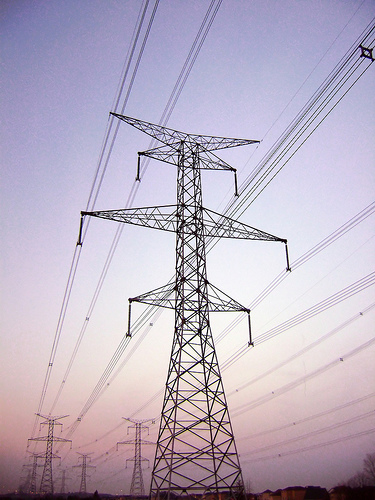
\includegraphics[scale=0.15]{arescue-figures/ElectricGrid.jpg}  \\
                \textcolor{purple}{Electricity Grid}
                \end{tabular}
            \column{0.33\textwidth}
                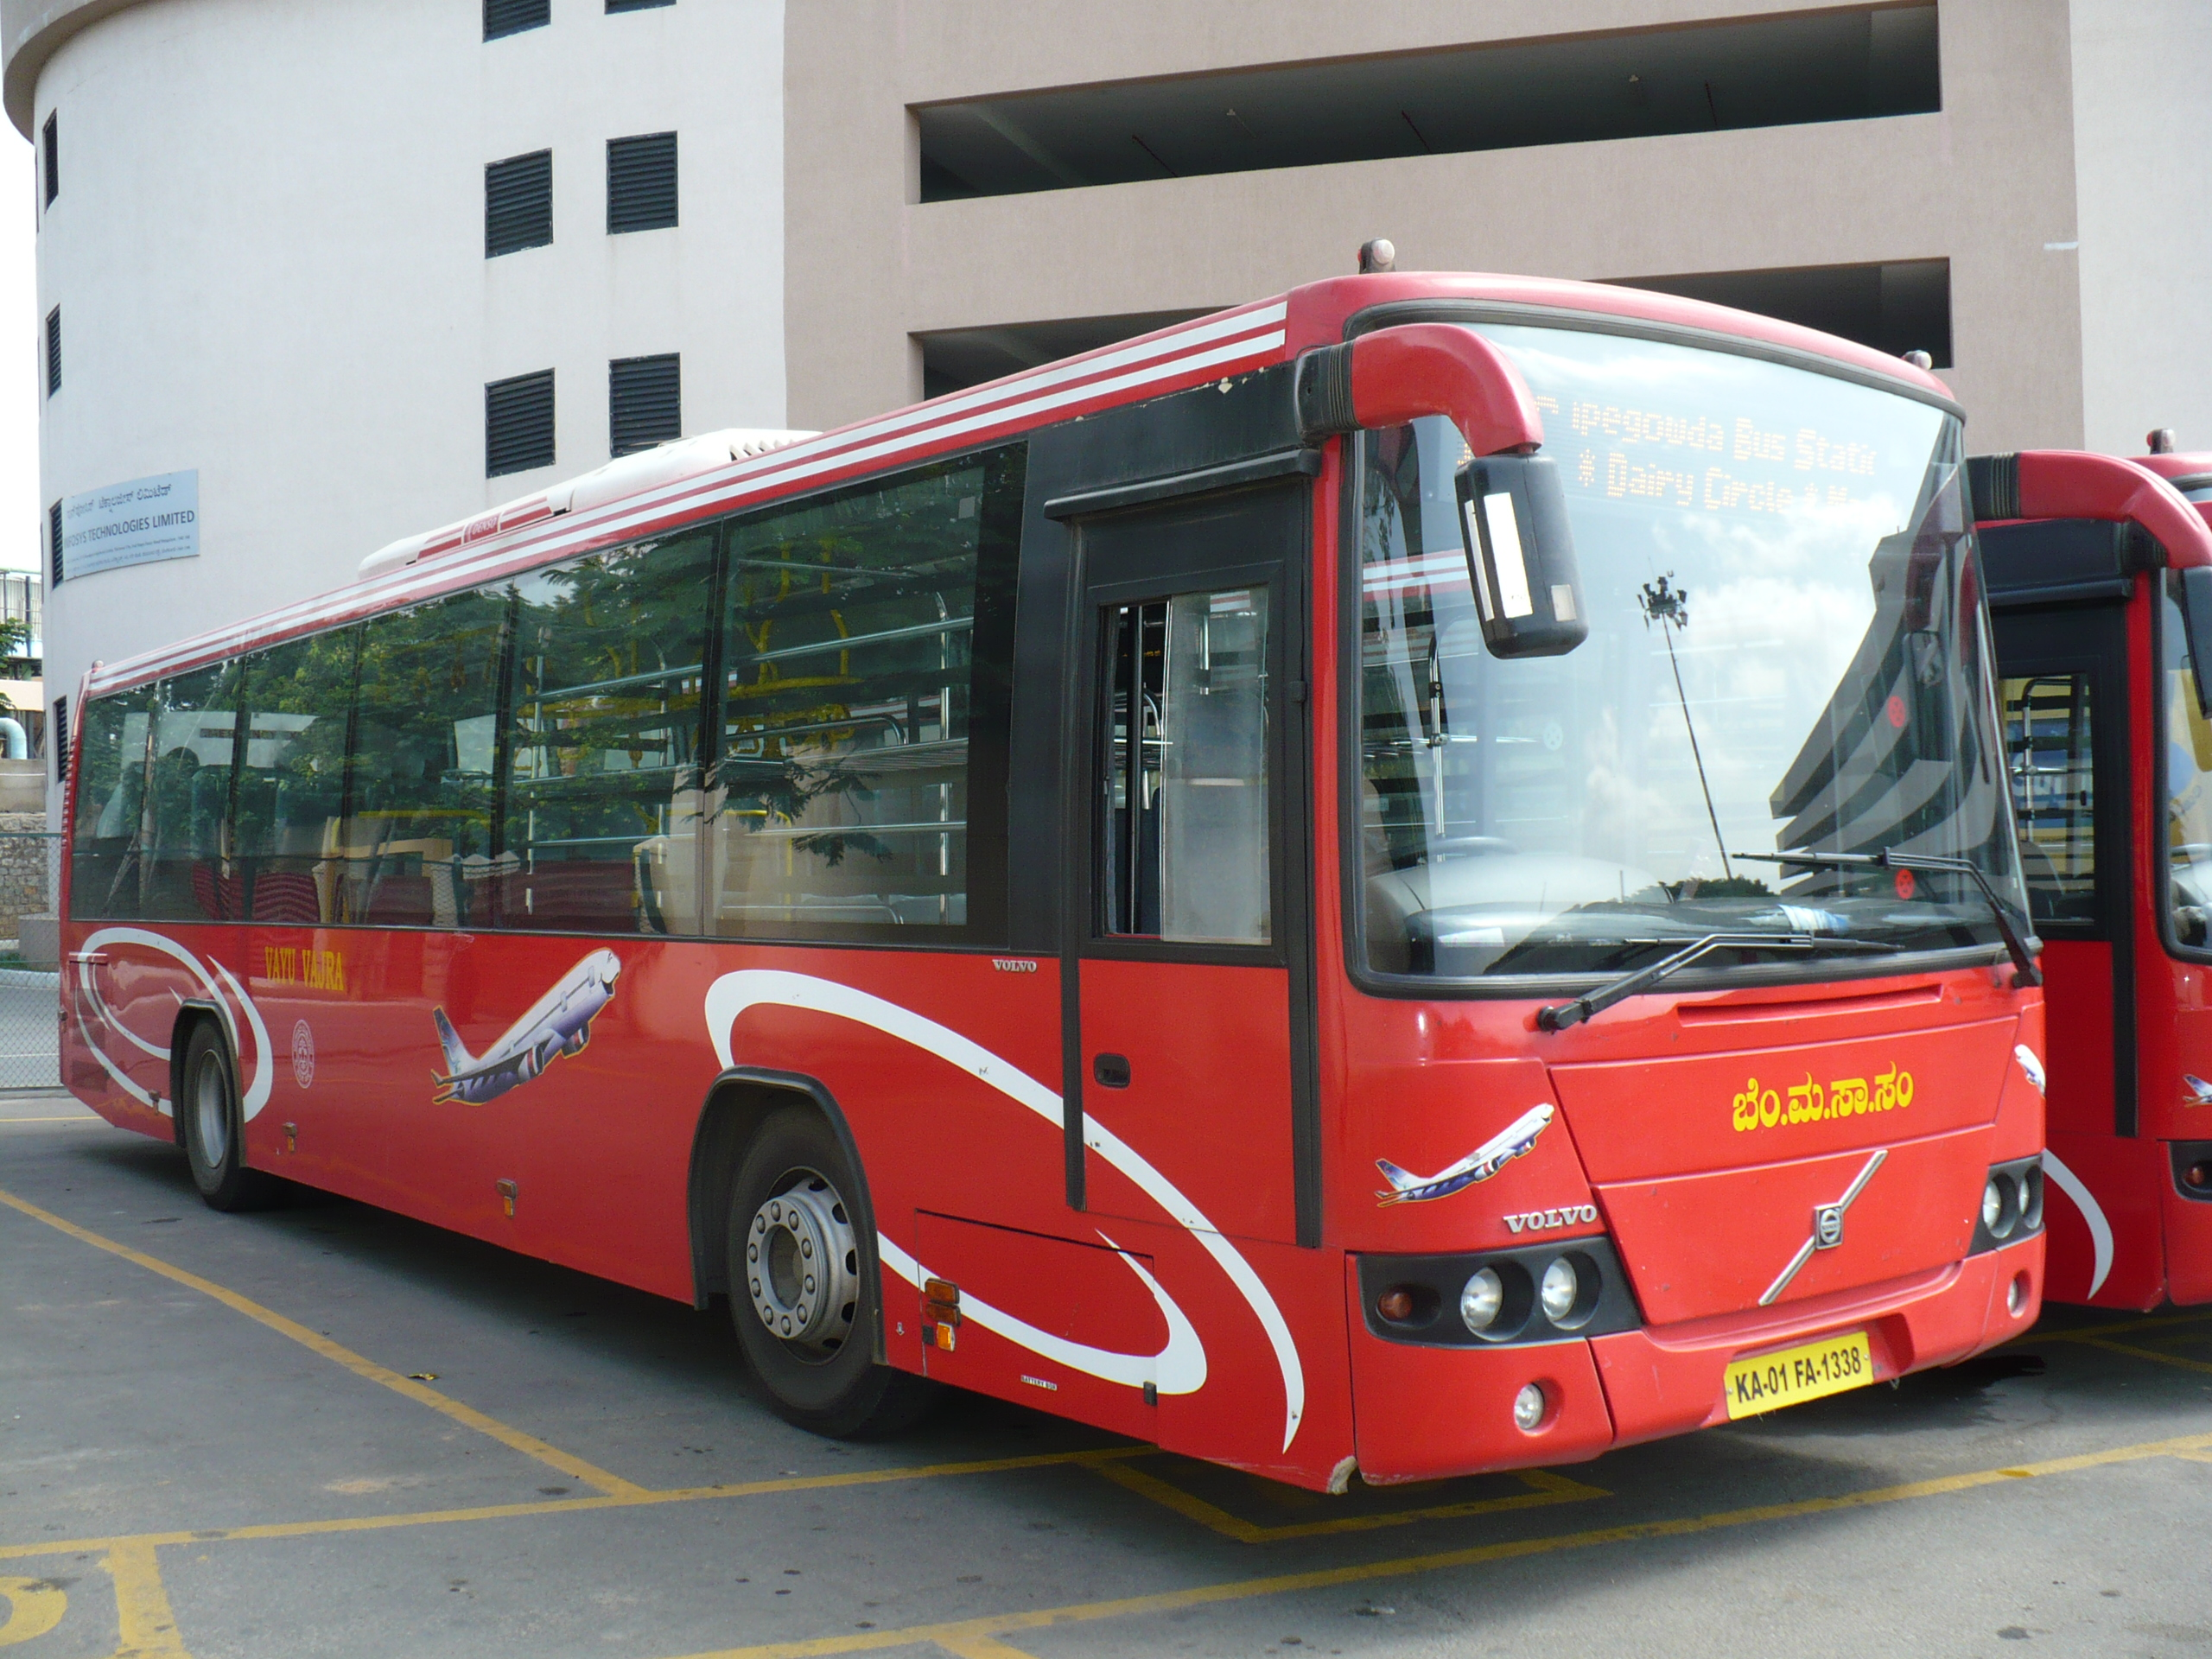
\includegraphics[scale=0.035]{arescue-figures/Bangalore-Public-Transport.jpg} \\
                \textcolor{purple}{Public Transport}
            \column{0.33\textwidth}
                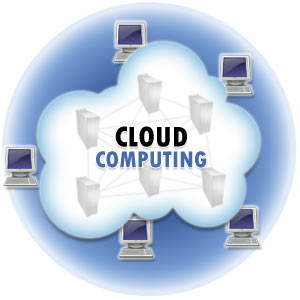
\includegraphics[scale=0.35]{arescue-figures/cloud.jpg} %\\
%               \textcolor{purple}{Cloud Computing}
        \end{columns}
    \pause
    \begin{columns}
        \column{0.6\textwidth}

        \column{0.4\textwidth}
        \begin{block}{}
            \begin{itemize}
            \item Software as a Service
            \item Platform as a Service
            \item Infrastructure as a Service
            \end{itemize}
        \end{block}

    \end{columns}

    \begin{textblock*}{100mm}[0,0](14.5mm,20mm)
        \begin{tikzpicture}[overlay]
%           \node[rectangle] (a) at (0.5,-6) {};
%           \node[rectangle,color=blue] (b) at (7,-4.5) {Virtualization};
%           \path[->, color=blue, line width=0.5mm]<1-> (a) edge [bend right] (b); %node[midway,below] {Abstraction};
%           \path [decorate,decoration={text along path, text={Resource Abstraction}}] (3,-6.3) to[bend right] (7,-4);%(0.5,-6) -- (7,-4.5);
            \node[coordinate] (a) at (2,-6) {};
            \node[coordinate] (b) at (7,-6) {};
            \node[rectangle,color=blue] (c) at (0.7,-6) {Virtualization};
            \begin{scope}
                \pgfsetlinewidth{2pt}
                \draw[->,color=blue] (b) -- (a) node[midway,above,black] {Enabling technology};
            \end{scope}
        \end{tikzpicture}
    \end{textblock*}

    \end{frame}

%Nice slide but commented for pre-syn purposes
%     %%%%%%%%%%%%% SLIDE %%%%%%%%%%%%%%  
%       \subsection{IaaS via Virtualization}
%     \begin{frame}[shrink]
%         \frametitle{Infrastructure as a Service (IaaS) via Virtualization}
% \vspace{0.1in}
%          \begin{textblock*}{100mm}[0,0](9.5mm,15mm)
%             \begin{varblock}[4.5cm]{}
%             Virtualization Architecture
%             \end{varblock}
%         \end{textblock*}
% 
%         \noindent\makebox[\textwidth]{% check this SSS........
%          \begin{columns}
%             \column{0.5\textwidth}
% \vspace{0.1in}
%             \noindent\makebox[\textwidth]{%         
% %           \begin{tabular}{c}
%             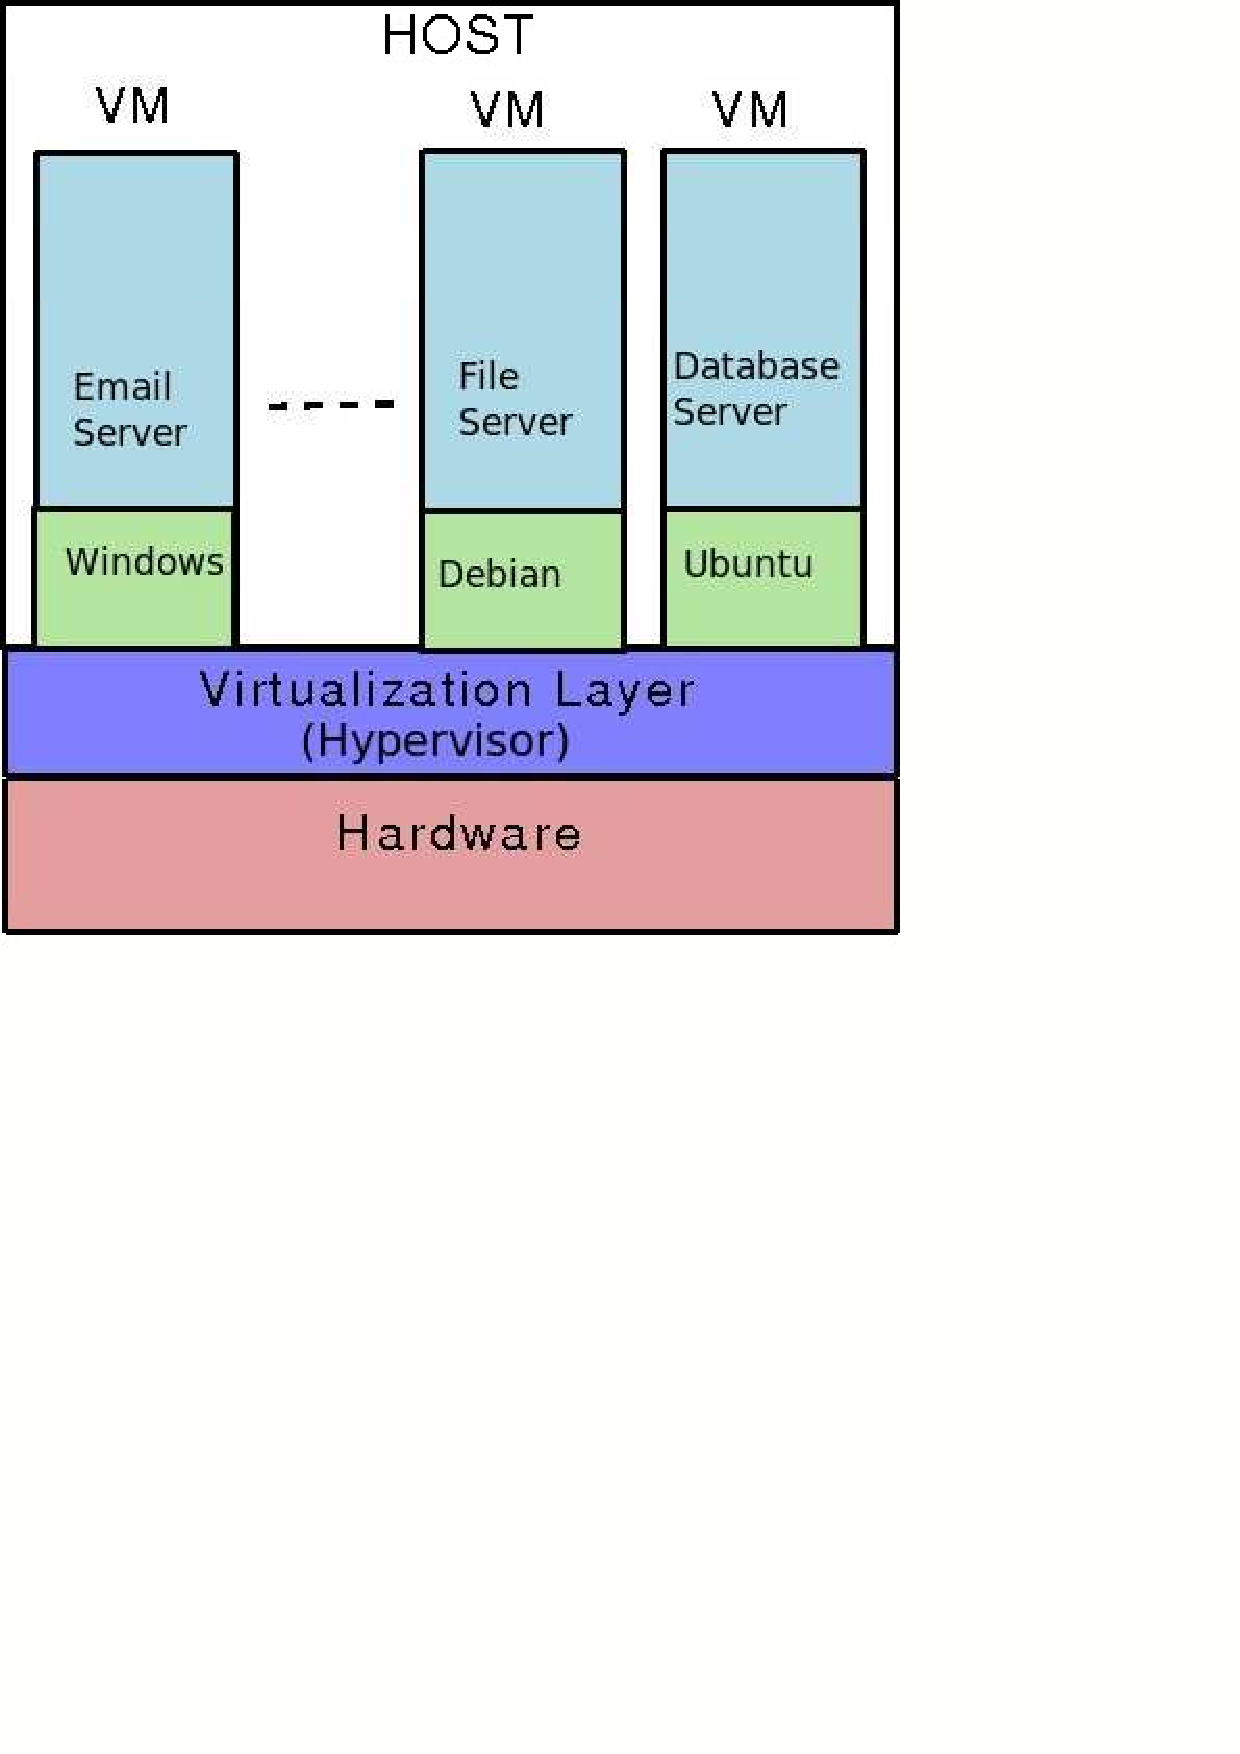
\includegraphics[scale=0.25]{arescue-figures/intro-diag.pdf} %\\
% %           \textcolor{purple}{$Fig: $}Virtualization Architecture %\\
%             % 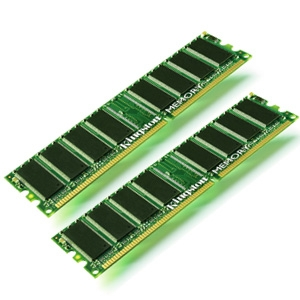
\includegraphics[scale=0.1]{figures/RAM.jpg}
% %           \end{tabular}
%             }
% \vspace{-1.6in}
%             \begin{block}{Enables}
%              \begin{itemize}
%               \item De-coupling hardware \& software
% %             \item On-demand resource allocation
%             \item Multiplexing of resources
%             \item Machine-level on-demand resource allocation
%              \end{itemize}
% 
%             \end{block}
% 
%             \column{0.5\textwidth}
%             \begin{exampleblock}{Benefits for Users}
%              \begin{itemize}
%               \item Pay-per-use
% %           \item No hardware maintenance burden
%             \item Infrastructure management outsourced
% %           \item Assured QoS (as per SLAs)
%             \item Performance guarantees and isolation
% 
%              \end{itemize}
%             \end{exampleblock}
% 
% 
%             \begin{exampleblock}{Benefits for Providers}
%              \begin{itemize}
% %             \item Reduction in server sprawl by employing multi-cores
%             \item Multiplex resources for operating efficiency
%             \item Enable server consolidation => reduced server sprawl
%             \item Optimize power and cooling costs%; proportional to user base
%              \end{itemize}
%             \end{exampleblock}
% 
%         \end{columns}}
%     \end{frame}
    
% 	%%%%%%%%%%%%% SLIDE %%%%%%%%%%%%%%
% 	\begin{frame}
% 	  \frametitle{Virtual Machine Relations}
% 	  
% 	  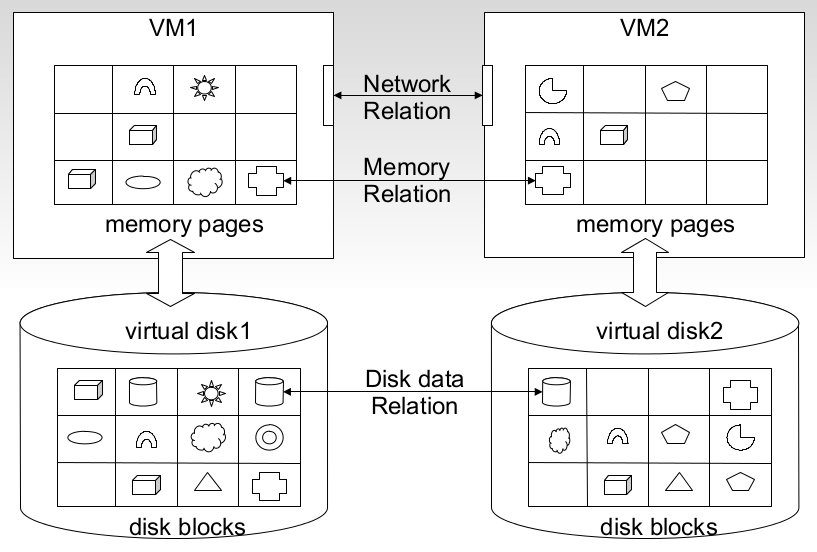
\includegraphics[scale=0.275]{sixth-aps-figures/vm-relations.jpg}
% 	      \begin{block}{}
% 		\scriptsize
% 		\begin{itemize}
% 		    \item Network relation refers to network traffic between virtual machines. 
% 		    \item Both the memory and disk data relations are based
% 			on data-similarity => \textit{data-similarity relation}
% 		    \item \textcolor{darkgreen}{In this talk, we focus on the data-similarity relation.}
% 		\end{itemize}
% 	      \end{block}
% 	\end{frame}
    
    %%%%%%%%%%%% SLIDE %%%%%%%%%%%%%%    
    \subsection{Virtualized Resources}
    \begin{frame}
	\frametitle{Thesis Scope}
% 	\vspace{-0.5in}
	\begin{block}{Two types of resources in virtualized environment}
	 \begin{enumerate}
	  \item Resources allocated to virtual machines
	  \item Resources available to host for virtualization operation \& overheads
	 \end{enumerate}

	\end{block}

% %         \begin{columns}
% %             \column{0.45\textwidth}
                \begin{figure}%[t]
%                 \centering
%                 \vspace{-0.2in}
                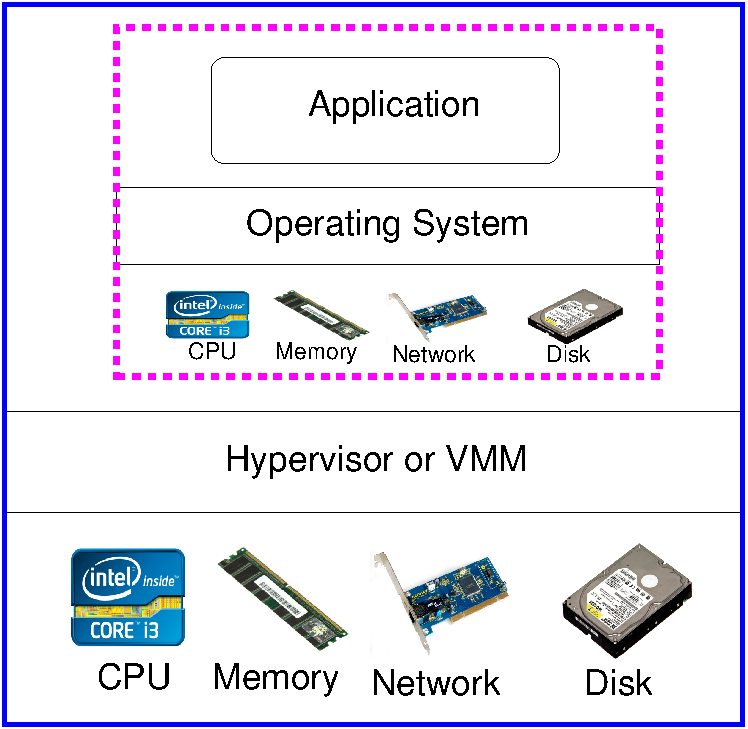
\includegraphics[scale=0.45]{presyn-figures/resource-types.pdf} %\\
                \end{figure}	

        \only<2->{
        \begin{tikzpicture}[overlay]
        \node[rectangle,color=purple] at (1.75,5.25) {Thesis};
        \node[rectangle,color=purple] at (1.05,4.75) {Component \#1};

        \begin{scope}
        \pgfsetlinewidth{1pt}
            \node[coordinate] (a) at (2.25, 5) {};
            \node[coordinate] (b) at (6.25, 4) {};
            \node[coordinate] (c) at (4.35, 3.95) {};
            \node[coordinate] (d) at (3.95, 2.1) {};

        \pgfsetlinewidth{2pt}
            \draw[->,style=dotted,color=purple] (a) -- (b);
            \draw[->,style=dotted,color=purple] (a) -- (c);
            \draw[->,style=dotted,color=purple] (a) -- (d);

        \end{scope}
        \end{tikzpicture}                
                
        \begin{tikzpicture}[overlay]
        \node[rectangle,color=blue] at (10.75,5.25) {Thesis};
        \node[rectangle,color=blue] at (10.95,4.75) {Component \#2};

        \begin{scope}
        \pgfsetlinewidth{1pt}
            \node[coordinate] (p) at (10.25, 4.5) {};
            \node[coordinate] (q) at (8, 4.3) {};
            \node[coordinate] (r) at (5.25, 2.5) {};
            \node[coordinate] (s) at (8.25, 2.4) {};

        \pgfsetlinewidth{2pt}
            \draw[->,style=dotted,color=blue] (p) -- (q);
            \draw[->,style=dotted,color=blue] (p) -- (r);
            \draw[->,style=dotted,color=blue] (p) -- (s);

        \end{scope}
        \end{tikzpicture}
        }

    \end{frame}

    
%Add thesis scope in previous slide itself    
%     %%%%%%%%%%%%% SLIDE %%%%%%%%%%%%%%
%       \subsection{Thesis Scope}
%     \begin{frame}
% 	\begin{block}{Thesis Scope}
% 	 sdfsd
% 	\end{block}
% 
%     \end{frame}

    %%%%%%%%%%%%% SLIDE %%%%%%%%%%%%%%
    \section{Thesis Contributions and Challenges within}
    \begin{frame}
	\frametitle{Top 3 Contributions}
	
% 	\scriptsize
      \vspace{-0.2in}
      \begin{block}{Contribution 1: Network-affinity aware CPU Usage Estimation}
	        \begin{itemize}
	        \item \textit{Initial Attempt:} Linear model 
% 	        based on multiple resource usage profiles 
	        to predict ``total'' CPU requirement
	        \item \textit{Challenge:} Maximum error 5-6\% absolute CPU
	        \item \textit{How Overcame:} Predict ``differential'' CPU usage---Max error 1-2\% 
% 	        \item \textit{Final Outcome:}
	       \end{itemize}
      \end{block}
      \begin{block}{Contribution 2: VM Disk I/O Reduction by Host-cache Manipulation}
	    \begin{itemize}
	        \item \textit{Initial Attempt:} Performing variable-sized deduplication
	        \item \textit{Challenge:} Real-world trace available only for fixed-size, not variable
	        \item \textit{How Overcame:} Show value of caching hints in fixed-size dedup
% 	        \item \textit{Final Outcome:}
	    \end{itemize}
      \end{block}
      \begin{block}{Contribution 3: I/O trace characterization for deduplication}
	 \begin{itemize}
	        \item \textit{Initial Attempt:} I/O tracing toolkit but no production tracing
	        \item \textit{Challenge:} Need real workloads/realistic traces for characterization
	        \item \textit{How Overcame:} Extensive dataset %\& literature 
		    survey to make the \textit{case} that need to generate 
		    realistic I/O traces with content representation
	 \end{itemize}

	\end{block}

    \end{frame}
% 
%     %%%%%%%%%%% SLIDE %%%%%%%%%%%%%%
%     %http://compgroups.net/comp.text.tex/chapters-in-beamer/1911862
%     \part{Affinity-aware Modeling of CPU Usage for Provisioning Virtualized Applications}
%     \frame{\partpage\strut}
%         

    %%%%%%%%%%%%% SLIDE %%%%%%%%%%%%%%
    \begin{frame}
	\frametitle{Content Outline---Part I}
	    \begin{block}{Affinity-aware CPU usage estimation in \textit{migratory} VM scenarios}
	    \begin{enumerate}
	     \item \textcolor{magenta}{Profiling study} of Xen network virtualization to 
		  show the different flow paths for \textit{intra-PM} 
		  and \textit{inter-PM} network traffic
	     \item \textcolor{magenta}{Benchmarking} of CPU usage for various workloads
		  in colocated and dispersed scenarios (demonstrated to be linear)	     
	     \item Pair-wise linear regression model to \textcolor{magenta}{predict total} CPU when network traffic 
		  changes nature between intra-PM and inter-PM
	     \item Pair-wise linear regression model to \textcolor{magenta}{predict differential} CPU usage 
	     \item Application of pair-wise models to predict for \textcolor{magenta}{multi-VM scenarios}
	    \end{enumerate}
	    \end{block}

	   \begin{exampleblock}{Tools and deliverables}
	  \begin{itemize}
	   \item \texttt{WLoadGen:} A load generator for CPU, disk \& network loads
	  \end{itemize}
	  \end{exampleblock}
	  
    \end{frame}

%%%%%%%%%%%% SLIDE %%%%%%%%%%%%%%
    \section{Motivation}
    \begin{frame}%[shrink]
    \frametitle{Migration-Enabled Resource/Performance Management}
        \vspace{-0.15in}
        \begin{varblock}[8.5cm]{}
%       Migration for consolidation
        \textcolor{magenta}{Consolidate/colocate} VMs for Resource Efficiency
        \end{varblock}

        \begin{figure}%[t]
        \centering
        \vspace{-0.2in}
        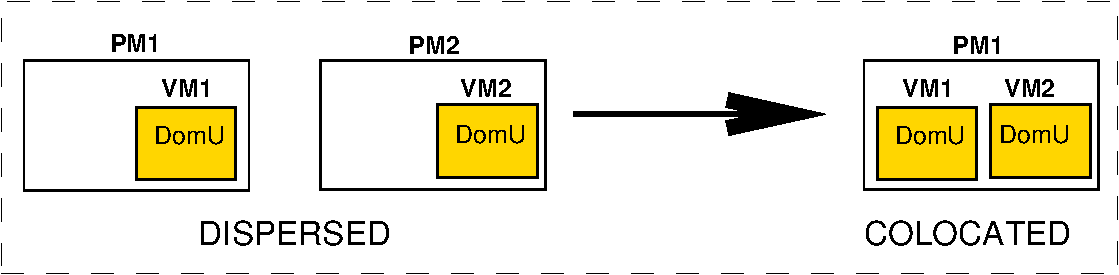
\includegraphics[scale=0.35]{arescue-figures/disp-to-colo.pdf} %\\
        \end{figure}

        \vspace{-0.15in}
        \begin{varblock}[6.5cm]{}
%       Migration for QoS
        \textcolor{magenta}{De-consolidate/disperse} VMs for QoS
        \end{varblock}

        \begin{figure}%[t]
        \centering
        \vspace{-0.2in}
        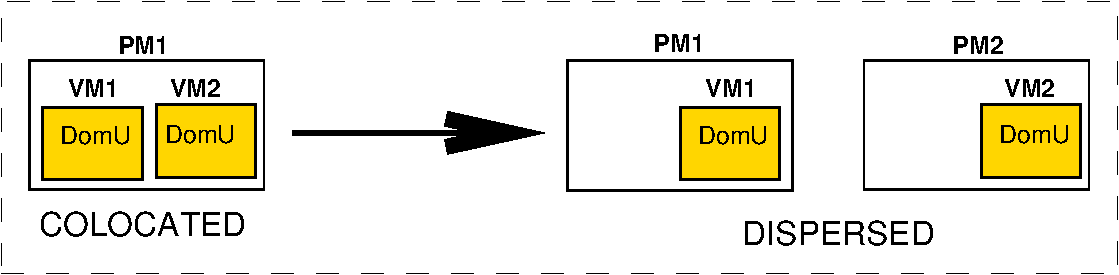
\includegraphics[scale=0.35]{arescue-figures/colo-to-disp.pdf}
        \end{figure}

        \begin{block}{}
            \begin{itemize}
%           \item Each case requires resource usage estimation - based on load and SLA 
            \item Both colocation and dispersion need \textcolor{magenta}{resource usage estimation}
            \item Incorrect estimation is sub-optimal
            \begin{itemize}
                \item Under-estimation => degraded performance
                \item Over-estimation => wasted resources
            \end{itemize}
            
%           \item Our argument: Ignoring affinity might result in improper estimation
            \end{itemize}
        \end{block}

    \end{frame}        

        %%%%%%%%%%%%% SLIDE %%%%%%%%%%%%%%
    \frame{
        \frametitle{Mutable and Immutable Network traffic for \textit{Migratory} VMs}
% \vspace{-0.2in}
\begin{tikzpicture}
\node[text height=2cm, text width=2cm, draw, rectangle] (a) at (9,10) {};
\node[text height=2cm, rectangle,color=purple] (b) at (9,10) {VM1};
\node[text height=2cm, rectangle] (c) at (6,10) {};
\node[text height=2cm, text width=2cm, draw, rectangle] (d) at (14,10) {};
\node[text height=2cm, rectangle,color=purple] (e) at (14,10) {VM2};
\node[text height=2cm, rectangle] (f) at (17,10) {};
\node[text height=2cm, color=purple, rectangle] at (9,11) {Web tier};
\node[text height=2cm, color=purple, rectangle] at (14,11) {Database tier};
\node[text height=2cm, color=blue, rectangle] (x) at (7,10) {n/w};
\node[text height=2cm, color=blue, rectangle] (x2) at (16,10) {n/w};
\node[text height=2cm, color=blue, rectangle] (y) at (7,9.5) {traffic};
\node[text height=2cm, color=blue, rectangle] (y2) at (16,9.5) {traffic};
\node[text height=2cm, color=blue, rectangle] (z) at (11.5,10) {traffic};

\begin{scope}
     \pgfsetlinewidth{2pt}
\draw[<->,color=blue] (a) -- (c) node[midway,above] {Req/Res} node[midway,below] {Immutable};
\draw[<->,color=blue] (d) -- (f) node[midway,below] {Immutable};
\draw[<->,color=blue] (a) -- (d) node[midway,above] {DB query} node[midway,below] {Mutable n/w};
% \draw[->,color=blue] (b) -- (d);
% \draw[->,color=blue] (c) -- (d);
% \draw[->,color=blue] (d) -- (e);
% \node[text height=2cm, color=blue, rectangle] at (6.5,11.5) {Intra-PM};
% \node[text height=2cm, color=blue, rectangle] at (6.5,11.5) {Inter-PM};
     \end{scope}

\end{tikzpicture}
% \end{block}
\vspace{0.1in}
\begin{block}{Mutable n/w traffic}
 Network traffic between VMs whose relative 
    placement may \textcolor{magenta}{\textit{change between colocated 
    and dispersed}}, due to server consolidation strategies
\end{block}

\vspace{-0.1in}
\begin{block}{Our hypothesis}
Mutable network traffic has \textcolor{magenta}{different CPU overheads} in 
colocated and dispersed scenarios => ignoring affinity effects 
could result in incorrect CPU usage estimation
\end{block}

}

%   %%%%%%%%%%% SLIDE %%%%%%%%%%%%%%
    \begin{frame}
        \frametitle{Communicating VMs (Xen-view)}
\vspace{-0.1in}
        \begin{columns}
            \column{0.85\textwidth}
                \begin{figure}%[t]
                \centering
                \vspace{-0.2in}
                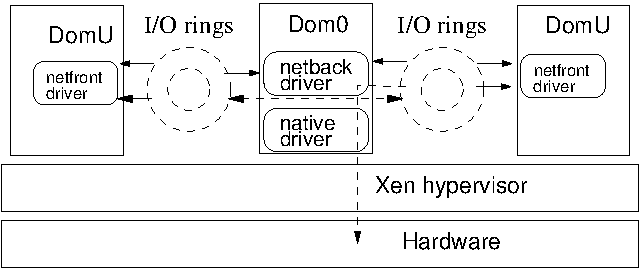
\includegraphics[scale=0.85]{arescue-figures/xenimpl.pdf} %\\
                \end{figure}
            \column{0.15\textwidth}
        \end{columns}

%       \pause
        \begin{textblock*}{100mm}[0,0](14.5mm,20mm)
            \begin{tikzpicture}[overlay]
                \node[rectangle] (a) at (0.5,-1.2) {};
                \node[rectangle] (b) at (7.5,-1.2) {};
                \node[rectangle,color=purple] (x) at (9.5,-1.2) {Intra-PM};
                \node[rectangle] (c) at (4,-3.5) {};
                \node[rectangle] (d) at (4,-2) {};
                \node[rectangle] (e) at (7.5,-2) {};
                \node[rectangle,color=blue] (x) at (9.5,-2) {Inter-PM};

                \begin{scope}
                    \pgfsetlinewidth{3pt}
                    \draw[<->,color=purple, style=dotted] (a) -- (b);% node[right,above] {Affine} node[right,below] {traffic};
                    \draw[<-,color=blue, style=dotted] (c) -- (d);% node[right,above] {Affine} node[right,below] {traffic};
                    \draw[->,color=blue, style=dotted] (d) -- (e);% node[right,above] {Affine} node[right,below] {traffic};
                \end{scope}

%               \path[->, color=blue, line width=0.5mm]<1-> (a) edge [bend right] (b); %node[midway,below] {Abstraction};
%               \path [decorate,decoration={text along path, text={Resource Abstraction}}] (3,-6.3) to[bend right] (7,-4);%(0.5,-6) -- (7,-4.5);

    %           \path[->]<2-> (n2) edge [bend right] (t2);
    %           \path[->]<3-> (n3) edge [out=0, in=-90] (t3);
            \end{tikzpicture}
        \end{textblock*}

%       \pause
        \begin{block}{}
        \begin{itemize}
    %        \item Among network loads, affine and non-affine network traffic have different CPU overheads.
    %       \item Different CPU overheads when VMs colocated and dispersed
            \item \textcolor{magenta}{Dom0 overhead} for DomU's I/O activity (network \& disk)
            \item Intra-PM network traffic
            \begin{itemize}
                \item Dom0 does not use native I/O drivers
                \item Shared memory based copying of packets
            \end{itemize}
            \item \textcolor{magenta}{Less CPU overhead for \textit{intra-PM}} traffic compared to \textit{inter-PM}
            \item Needs to be accounted for during VM migration
         \end{itemize}
        \end{block}
    \end{frame}

            
    %%%%%%%%%%%%% SLIDE %%%%%%%%%%%%%%
    \subsection{Benchmarking: Effect of colocation on CPU usage for Mutable N/w traffic}
    \frame{
        \frametitle{Benchmarking: Effect of colocation on CPU usage for \textit{Mutable} N/w traffic}

        \vspace{-0.15in}
        \begin{varblock}[12.0cm]{}
%       Migration for QoS
        \textcolor{magenta}{Benchmarking setup:} 2 VMs on 2 PMs---dispersed and colocated scenarios
        \textcolor{magenta}{Network load:} Transmitted (Tx) by one VM and Received (Rx) by other
        \end{varblock}
        
        \vspace{0.1in}
        \begin{columns}
            \column{0.5\textwidth}
            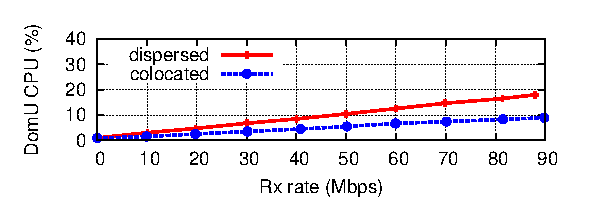
\includegraphics[scale=0.65]{arescue-figures/aff-benchmark/domU-cpu-vs-affine-rx-curve.eps} \\
            (a) Receiving DomU CPU util
            \column{0.55\textwidth}
            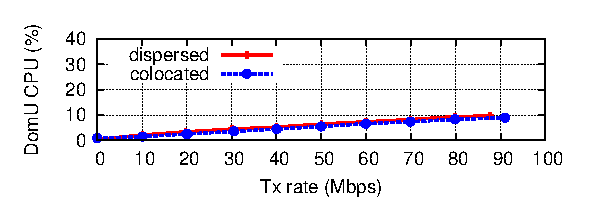
\includegraphics[scale=0.65]{arescue-figures/aff-benchmark/domU-cpu-vs-affine-tx-curve.eps} \\
            (b) Transmitting DomU CPU util
        \end{columns}
        \begin{columns}
            \column{0.5\textwidth}
            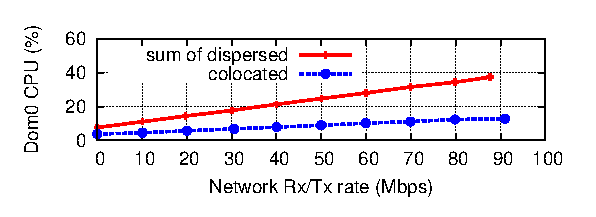
\includegraphics[scale=0.65]{arescue-figures/aff-benchmark/dom0-cpu-vs-affine-curve.eps} \\
            (c) Dom0 CPU util for Rx/Tx %(summation versus co-located)
            \column{0.55\textwidth}
            \begin{exampleblock}{Observations}
\begin{small}
             \begin{itemize}
              \item \textbf{DomU}: Rx increase from 20-90 Mbps =>decrease of 2-8\% CPU util
            \item \textbf{Dom0}: Increase from 20 to 90 Mbps =>decrease from 9-25\% CPU util %(summation of dispersed versus colocated)
             \end{itemize}
\end{small}
% \setbeamerfont{item}{size=\default}

            \end{exampleblock}

        \end{columns}
    }
    
    
    %%%%%%%%%%%%% SLIDE %%%%%%%%%%%%%%
    \subsection{Benchmarking: Effect of colocation on CPU usage for Immutable N/w traffic, CPU and disk loads}
    \frame{
        \frametitle{Benchmarking: Effect of colocation on CPU usage for Immutable n/w traffic, CPU and disk loads}

        \vspace{-0.1in}
        \begin{varblock}[12.0cm]{}
%       Migration for QoS
        \textcolor{magenta}{Benchmarking setup:} 4 VMs on 4 PMs---dispersed and colocated scenarios
%         \textcolor{magenta}{Workloads:} Immutable n/w traffic, CPU and disk read/write
        \end{varblock}
        
\vspace{-0.2in}        
\begin{table}
\centering
\caption{Percentage CPU usage for Immutable Rx}
% \noindent\makebox[\textwidth]{% 
\begin{tabular}{|c|c|c|} \hline
\textbf{Immutable} & \multicolumn{2}{|c|}{\textbf{\% CPU utilization}} \\ \cline{2-3} \cline{2-3}
\textbf{Rx} & \textbf{Dispersed case} & \textbf{Colocated case} \\
(Mbps) & $VM_1,VM_2, \sum Dom0_i$ & $VM_1,VM_2,Dom0$ \\ \hline
% $<$20, 10$>$ & 3, 2, 12 & 3, 2, ~8 \\ \hline
% $<$20, 30$>$ & 4, 5, 14 & 3, 5, 11 \\ \hline
$<$20, 50$>$ & 4, 7, 18 & 4, 7, 14 \\ \hline
% $<$20, 70$>$ & 4, 9, 21 & 4, 9, 17 \\ \hline
$<$40, 10$>$ & 6, 2, 15 & 6, 2, 11 \\ \hline
% $<$40, 30$>$ & 7, 5, 18 & 7, 5, 15 \\ \hline
% $<$40, 50$>$ & 7, 7, 21 & 7, 7, 18 \\ \hline
$<$60, 10$>$ & 8, 2, 18 & 8, 2, 14 \\ \hline
% $<$60, 30$>$ & 8, 5, 21 & 8, 5, 18 \\ \hline
\end{tabular}
% }
\label{nonaff-rx-benchmark}
\end{table}

    \begin{block}{Observations}% \& Summary of benchmarking}
	\begin{enumerate}
	 \item \textcolor{magenta}{No change in DomU CPU} usage between colocated and dispersed
	 \item Dom0 CPU usage change of \textcolor{magenta}{4\% for extra Dom0 instance (constant)}
	 \item \textcolor{magenta}{Similar observations for other workloads}---CPU and disk read/write
	\end{enumerate}

     
    \end{block}% \setbeamerfont{item}{size=\default}

    }

%%%%%%%%%%%%% SLIDE %%%%%%%%%%%%%%
    \section{Affinity-aware Modeling of CPU Usage}
    \subsection{Affinity-aware Resource Requirement Estimation}
    \begin{frame}
        \frametitle{Problem: Affinity-aware Resource Requirement Estimation}
% \vspace{-1.05in}
        \begin{alertblock}{}
%        Given a set of VMs and their resource utilization levels, to predict the CPU resource required by the VMs when co-located or dispersed.
        Given a pair of VMs and their resource utilization levels, predict the CPU resource requirement of DomU \& Dom0, 
        when VM placement scenario changes between dispersed and colocated.
        \end{alertblock}
%       this is wrong statement, it is not really an assumption. it is just that we need to learn model in unsaturated conditions
%       and also can be tested only on unsaturated conditions. however, when applying, initially all resources should be checked to
%       see if there is enough available, and then predict CPU usage. if enough CPU is available, then it implies unsaturated
%       and if not enough available, then migration should not be done. this ``assumption'' should be taken care of, by the
%       higher level consolidation or load balancing algorithm, it does not make any sense here.
%       \begin{alertblock}{Assumption}
%        Assumed that there are no resource bottlenecks or saturation.
%       \end{alertblock}

         \begin{columns}
            \begin{column}{0.4\textwidth}
%               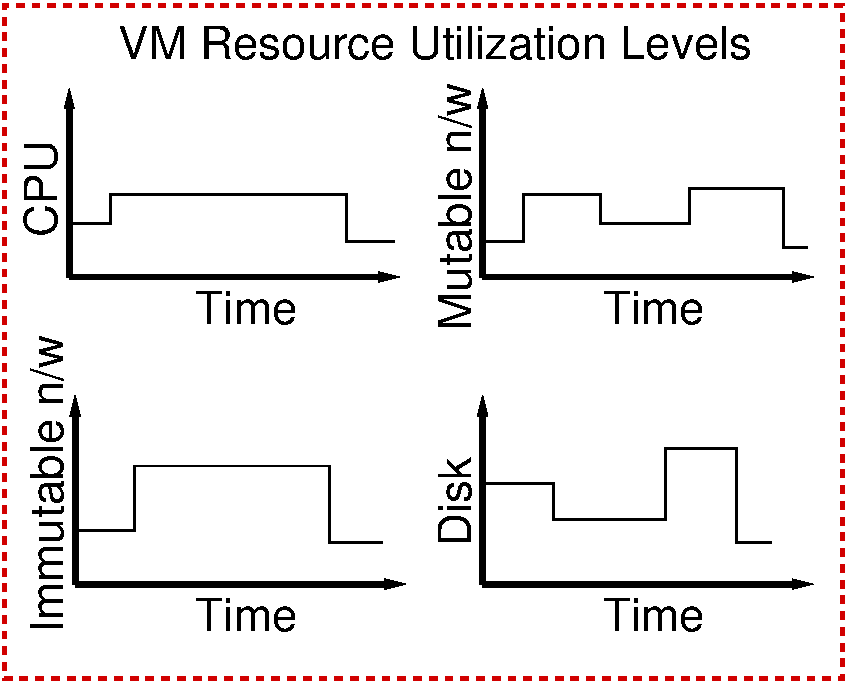
\includegraphics[height=4cm,width=5cm]{figures/dom1-app-traces.pdf}
                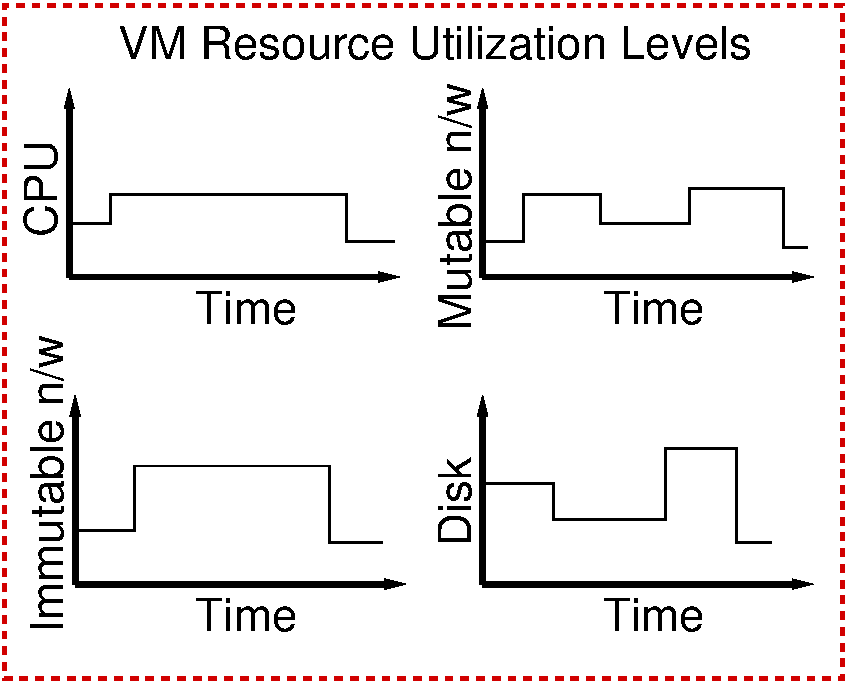
\includegraphics[scale=0.3]{figures/dom1-app-traces.pdf}
                \vspace{-0.1in}
                \begin{varblock}[5.0cm]{}
                 For VM1 and VM2 (dispersed)
                \end{varblock}

            \end{column}
            \begin{column}{0.2\textwidth}

            \end{column}
            \begin{column}{0.4\textwidth}
%               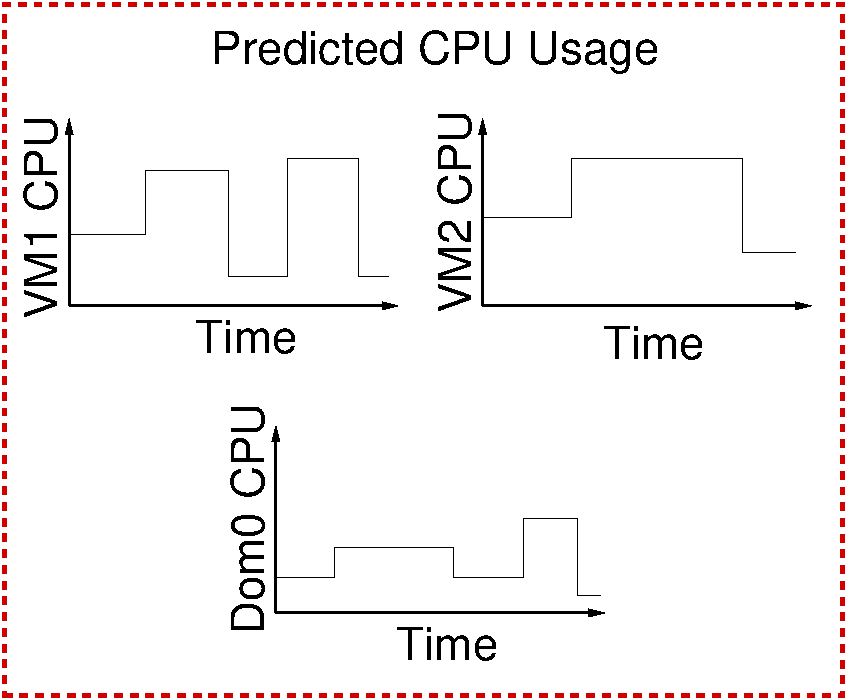
\includegraphics[height=4cm,width=5cm]{figures/virtual-app-traces.pdf}
                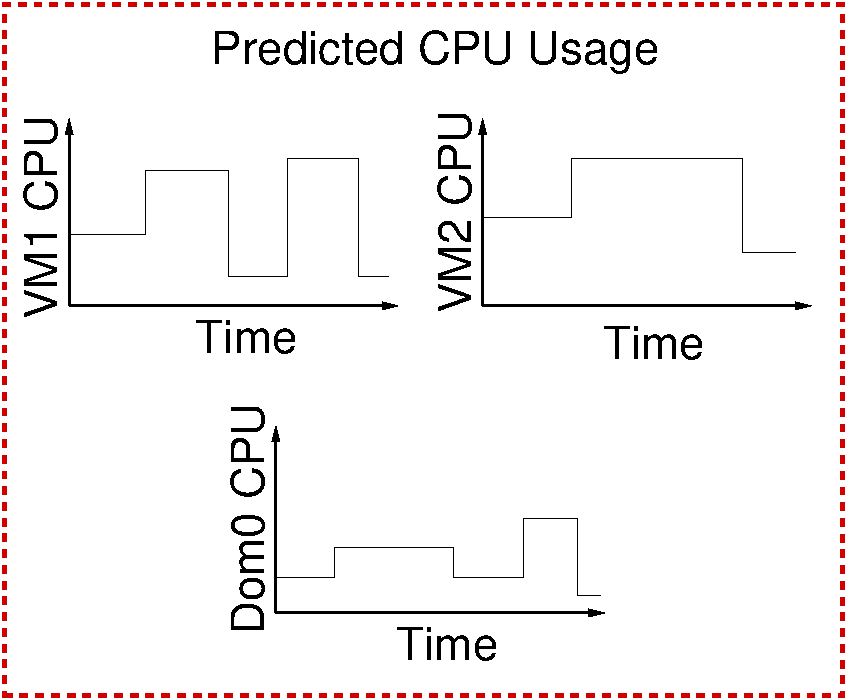
\includegraphics[scale=0.3]{figures/virtual-app-traces.pdf}
                \vspace{-0.1in}
                \begin{varblock}[3.0cm]{}
%                For VM1, VM2, Dom0 
                \centering
                (colocated)
                \end{varblock}
            \end{column}
        \end{columns}

        \begin{tikzpicture}[overlay]
%       \draw[step=1] (0,0) grid (13,13); 
% 	\node[rectangle,color=purple] at (5.5,3.75) {DomU \& Dom0};
        \node[rectangle,color=purple] at (5.5,3.25) {CPU usage};
        \node[rectangle,color=purple] at (5.5,2.75) {prediction};
        \node[rectangle,color=purple] at (5.5,2.25) {model};
        \begin{scope}
        \pgfsetlinewidth{1pt}
            \node[coordinate] (a) at (4.5, 3.75) {};
            \node[coordinate] (b) at (6.5,3.75) {};
            \node[coordinate] (c) at (6.5,1.75) {};
            \node[coordinate] (d) at (4.5,1.75) {};
%           \node[coordinate] (m) at (0,1) {};
%           \node[coordinate] (n) at (1.5,2.25) {};
            \draw[-,color=purple] (a) -- (b);% node[midway,above] {DB query};% node[midway,below] {Affine n/w};
            \draw[-,color=purple] (b) -- (c);% node[midway] {Req/Res};
            \draw[-,color=purple] (c) -- (d);
            \draw[-,color=purple] (d) -- (a);
        \pgfsetlinewidth{2pt}
            \node[coordinate] (e) at (3.75, 2.5) {};
            \node[coordinate] (f) at (4.5,2.5) {};
            \node[coordinate] (g) at (6.5,2.5) {};
            \node[coordinate] (h) at (7.5,2.5) {};
            \draw[->,color=purple] (e) -- (f);
            \draw[->,color=purple] (g) -- (h);

        \end{scope}

        \end{tikzpicture}
        
        \begin{exampleblock}{Core Idea}
	    Since correlation of CPU usage with all other resources usage is linear, build \textcolor{magenta}{linear prediction models}
        \end{exampleblock}


    \end{frame}
    
%%%%%%%%%%%% SLIDE
    \begin{frame}%[shrink]
        \frametitle{Linear Regression Modeling for CPU Estimation}
        \vspace{-0.1in}
%       \begin{block}{Premise}
%       \begin{itemize}
%       \item Virtualized CPU usage depends on resource (cpu, network, disk) usage 
%       \item CPU usage has linear correlation with resource usage
%       \end{itemize}
%       \end{block}
\begin{small}
%       \begin{block}{}
%        Given 2 VMs with resources --- CPU, disk, memory, network
%       \end{block}

%       \pause
        \begin{block}{Parameters in the models}
         \begin{itemize}
          \item \textbf{CPU} metrics: user, system, iowait
          \item \textbf{Disk} metrics: read blocks/second, write blocks/second
           \item \textbf{Mutable and immutable} network metrics: Rx and Tx Kbps
         \end{itemize}
        \end{block}

%       \pause
        \begin{exampleblock}{DomU Models}
        $CPU_{colocated} = f(\textcolor{blue}{CPU},\textcolor{blue}{Disk},\textcolor{blue}{Mutable},\textcolor{blue}{Immutable})_{dispersed}$
        $CPU_{dispersed} = f(\textcolor{blue}{CPU},\textcolor{blue}{Disk},\textcolor{blue}{Mutable},\textcolor{blue}{Immutable})_{colocated}$

%       where
%           \begin{description}
%            \item  i=1,2
%           \end{description}

        \end{exampleblock}

        \begin{exampleblock}{Dom0 Models}
        $CPU_{colo} = f(\textcolor{blue}{CPU_1},\textcolor{blue}{Disk_1},\textcolor{blue}{Mutable_1},\textcolor{blue}{Immutable_1},$ 
	 \textcolor{white}{.}~~~~~~~~~~~~~~~~$\textcolor{red}{CPU_2}, \textcolor{red}{Disk_2}, \textcolor{red}{Mutable_2}, \textcolor{red}{Immutable_2})_{disp}$
        $CPU_{disp} = f(\textcolor{blue}{CPU_1},\textcolor{blue}{Disk_1},\textcolor{blue}{Mutable_1},\textcolor{blue}{Immutable_1})_{col}$ %, \textcolor{red}{CPU_2}, \textcolor{red}{Disk_2}, \textcolor{red}{Aff_2}, \textcolor{red}{NonAff_2})_{col}$

%       where
%           \begin{description}
%            \item  i=1,2
%           \end{description}

        \end{exampleblock}

\end{small}
    \end{frame}
    
    %%%%%%%%%%%% SLIDE
    \frame{
        \frametitle{Prediction for Synthetic workloads - Xen Dom0 model}
        \noindent\makebox[\textwidth]{% check this SSS........
         \begin{columns}
            \column{0.5\textwidth}
                \centering
                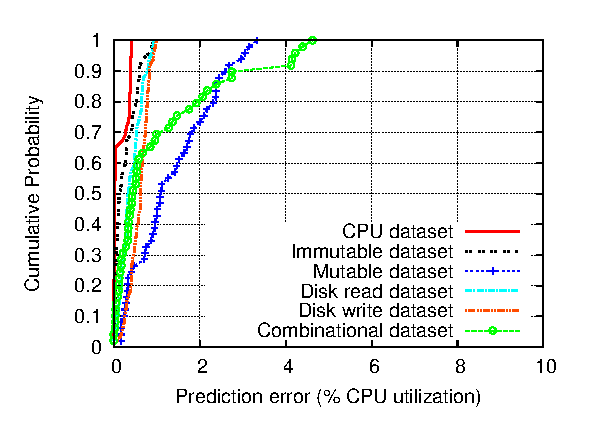
\includegraphics[height=4cm,width=5cm]{arescue-figures/synthetic-cdf-plots/dom0-forward-unseen-cdf-robust.eps} \\
                (a) Dispersed to colocated
            \column{0.5\textwidth}
                \centering
                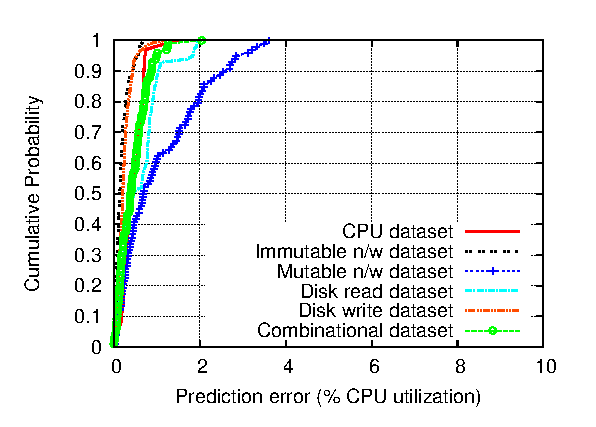
\includegraphics[height=4cm,width=5cm]{arescue-figures/synthetic-cdf-plots/dom0-reverse-unseen-cdf-robust.eps} \\
                (b) Colocated to dispersed
         \end{columns}
}
        \pause
        \begin{tikzpicture}[overlay]
            \node[coordinate] (a) at (0.25,4) {};
            \node[coordinate] (b) at (2.6,4) {};
            \node[coordinate] (d) at (2.6,1) {};

            \node[coordinate] (e) at (6.25,4) {};
            \node[coordinate] (f) at (8.45,4) {};
            \node[coordinate] (h) at (8.45,1) {};

            \begin{scope}
                \pgfsetlinewidth{2pt}
                \draw[-,style=dotted,color=purple] (a) -- (b);
                \draw[-,style=dotted,color=purple] (d) -- (b);
                \draw[-,style=dotted,color=purple] (e) -- (f);
                \draw[-,style=dotted,color=purple] (h) -- (f);
            \end{scope}
        \end{tikzpicture}

        \begin{exampleblock}{Observations}
         $90^{th}$ percentile prediction error within \textcolor{magenta}{3\% absolute CPU} utilization, 
         and maximum error 5-6\% absolute CPU 
         (Similarly for RUBiS workload as well)
        \end{exampleblock}
    }    
    

    
    %%%%%%%%%%%% SLIDE %%%%%%%%%%%%%%
    \begin{frame}
      \frametitle{Building an Enhanced Prediction Model}
      \begin{varblock}[12cm]{}
       \textcolor{magenta}{Because ``differential'' CPU usage is only due to mutable n/w traffic}
      \end{varblock}

      \begin{figure}
	  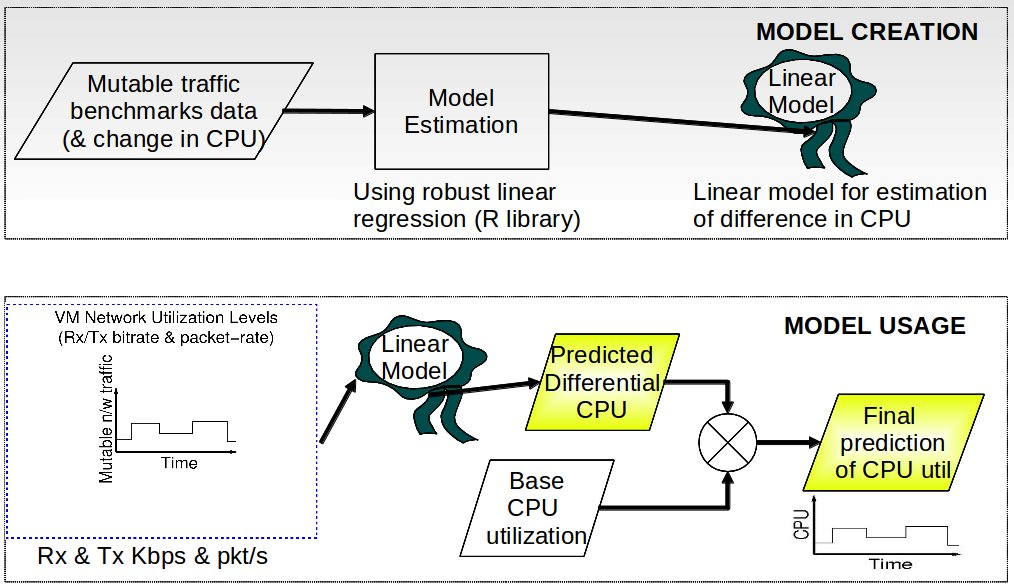
\includegraphics[scale=0.32]{arescue-figures/model-creation-usage.jpg}
      \end{figure}
      
%       \begin{block}{New input parameters}
% 	  Only metrics related to mutable network traffic
%       \end{block}
%       
%       \begin{block}{New output parameters}
% 	  Differential CPU usage instead of total usage
%       \end{block}


    \end{frame}

    %%%%%%%%%%%% SLIDE %%%%%%%%%%%%%%
    \begin{frame}{}
	\frametitle{Evaluation of Differential CPU Prediction Models}
	\vspace{-0.28in}
        \begin{columns}
            \begin{column}{0.5\textwidth}
	      \begin{figure}
		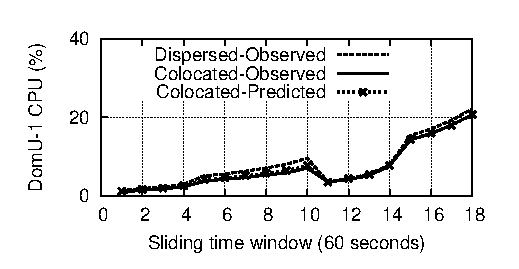
\includegraphics[scale=0.7]{jss-figures/aff-synth/synth-co-domu1.eps}
		\vspace{-0.1in}
		\caption{Colocated DomU-1 (Synthetic)}
	      \end{figure}
            \end{column}
            \begin{column}{0.5\textwidth}
	      \begin{figure}
		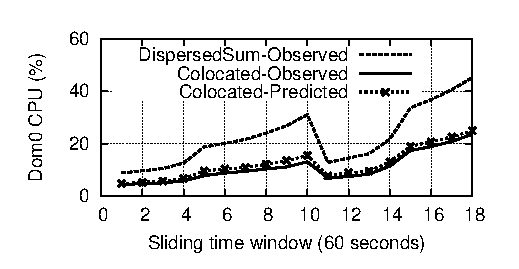
\includegraphics[scale=0.7]{jss-figures/aff-synth/synth-co-dom0.eps}
		\vspace{-0.1in}
		\caption{Colocated Dom0 (Synthetic)}		
	      \end{figure}             
            \end{column}
	\end{columns}

	\vspace{-0.25in}	
        \begin{columns}
            \begin{column}{0.5\textwidth}
	      \begin{figure}
		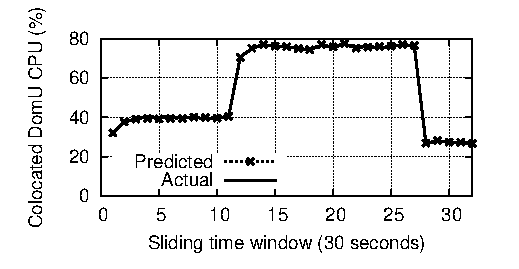
\includegraphics[scale=0.7]{jss-figures/aff-apps/rubis-co-domu1.eps}
		\vspace{-0.1in}
		\caption{Colocated DomU-1 (RUBiS)}		
	      \end{figure}             
            \end{column}
            \begin{column}{0.5\textwidth}
	      \begin{figure}
		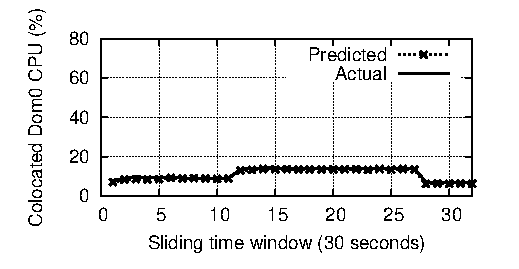
\includegraphics[scale=0.7]{jss-figures/aff-apps/rubis-co-dom0.eps}
		\vspace{-0.1in}
		\caption{Colocated Dom0 (RUBiS)}		
	      \end{figure}             
            \end{column}
	\end{columns}     

    \begin{exampleblock}{Result}
     Maximum prediction error between 1-2\% absolute CPU utilization.
    \end{exampleblock}	
 
 \end{frame}
    
   %%%%%%%%%%%% SLIDE %%%%%%%%%%%%%%
  \begin{frame}
    \frametitle{Applying Pair-wise Models to Multi-VM Scenarios}
    \vspace{-0.3in}
	      \begin{figure}
		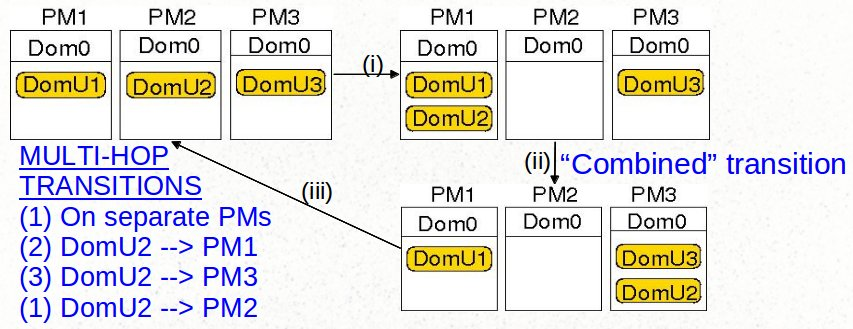
\includegraphics[scale=0.4]{jss-figures/multi-hop.jpg}
	      \end{figure}       
	      
\vspace{-0.25in}	      
\begin{table}[t]
\centering
\caption{Maximum error in Dom0 CPU utilization prediction}
% \noindent\makebox[\textwidth]{%
\begin{tabular}{ |c|c|c|c|} \hline
\textbf{Transition} & \multicolumn{3}{|c|}{\textbf{Max error (\% absolute CPU)}} \\ \cline{2-4}
%  & \multicolumn{3}{|c|}{\textbf{in Dom0 prediction}} \\ 
%  & \multicolumn{3}{|c|}{\textbf{(\% absolute CPU)}} \\ \cline{2-4}
 & \textbf{Dom0-PM1} & \textbf{Dom0-PM2}  & \textbf{Dom0-PM3} \\ \hline  %\cline{2-9}
Transition (i) & 0.75 & - & - \\
Transition (ii) & 1.99 & - & 0.85 \\
Transition (iii) & - & 0.51 & 0.43  \\ \hline
\end{tabular}
% }
\label{tab:vm-steps-error}
\end{table}
	      
  \end{frame}

    %%%%%%%%%%% SLIDE %%%%%%%%%%%%%%
    \begin{frame}
	\frametitle{Summary of Part I}

        \begin{itemize}
%        \item CPU requirement of communicating VMs can change upon VM migration.
        \item \textbf{Colocation of mutually-communicating VMs impacts their CPU requirement}
        \begin{itemize}
              \item \textcolor{purple}{DomU:} For Rx, increase from 20 to 90 Mbps => decrease from 2\% to 8\% CPU requirement
            \item \textcolor{purple}{Dom0:} Increase from 20 to 90 Mbps => decrease from 9\% to 25\% CPU requirement % (summation of dispersed Dom0 util compared to colocated)
        \end{itemize}

        \item \textbf{Simple linear model shown to predict ``differential'' CPU requirement from mutable n/w traffic profiles}
        \begin{itemize}
            \item \textcolor{purple}{Synthetic workloads:} Max error within 1.5\% absolute CPU utilization for both DomU and Dom0 models
            \item \textcolor{purple}{RUBiS benchmark application:} Max error within 1.5\% for Web and DB tiers, and Dom0
            \item \textcolor{purple}{Multi-VM scenario:} Max error within 2\% for all transitions
        \end{itemize}
        \end{itemize}
      
	
    \end{frame}


     
    %%%%%%%%%%%% SLIDE %%%%%%%%%%%%%%
%       \subsection{Part II}
    \begin{frame}
	\frametitle{Content Outline---Part II}
	    \begin{block}{Part II. Host cache usage optimization for virtualized services}
	      \begin{enumerate}
	      \item \textcolor{magenta}{Analysis of existing work (IODEDUP)} to show inconsistent performance
	       \item \textcolor{magenta}{Redirection} of I/O requests from within the virtual machines
	       \item To implicitly manipulate host cache in \textcolor{magenta}{content-deduplicated} fashion
	       \item Using \textcolor{magenta}{implicit caching hints}
	       \item Evaluation using public dataset available online%~\cite{iodedup-online}
	       \item \textcolor{magenta}{Case for generation} of realistic I/O deduplication benchmarks
	      \end{enumerate}
	    \end{block}
	
	\vspace{0.2in}
	\begin{exampleblock}{Tools and Deliverables}
	  \begin{enumerate}
% 	   \item \texttt{WLoadGen:} A load generator for CPU, disk \& network loads
	   \item \texttt{SimReplay}: A simulator for analyzing host cache effectiveness
	   \item \texttt{preadwritedump}: A kernel module for I/O request tracing
	  \end{enumerate}

	\end{exampleblock}
    \end{frame}	
    
    %%%%%%%%%%%%% SLIDE %%%%%%%%%%%%%%
    \frame[shrink]{
        \frametitle{Effect of Data Similarity on Host-cache Effectiveness}
        \begin{columns}
            \column{0.4\textwidth}
		  \vspace{-0.1in}
                \begin{figure}
                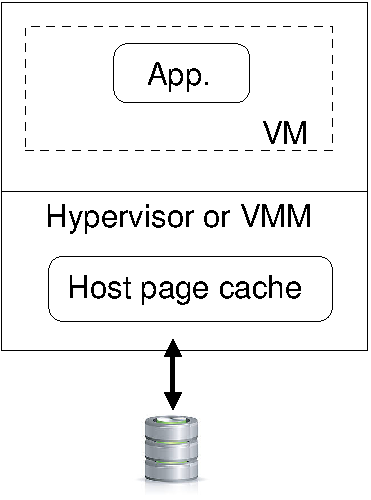
\includegraphics[scale=0.55]{confided-figures/main/system-under-considerat.pdf}
                \setbeamerfont{caption name}{size=\scriptsize}
                \setbeamerfont{caption}{size=\scriptsize}
                \vspace{-0.2in}
                \caption{Typical virtualized system}
                \end{figure}
                
                \begin{block}{Sources of data similarity}
		    Similar operating systems, libraries, binaries, file copies, etc.
                \end{block}

            \column{0.55\textwidth}
		\vspace{-0.1in}
                \begin{alertblock}{Two optimization avenues}
                    \begin{enumerate}
%                     \scriptsize
                        \item \textcolor{black}{Duplicate I/O}%: Multiple disk reads for same content in distinct blocks
                        \item \textcolor{black}{Duplicate content in cache}%: Duplicate content present in cache
                    \end{enumerate}
                \end{alertblock}

                \begin{alertblock}{Two orthogonal solutions}
                    \begin{enumerate}
%                     \scriptsize
                    \item \textcolor{blue}{I/O deduplication} (IODEDUP\cite{iodedup}) : but causes \textcolor{red}{cache inclusiveness problem}
%                     to eliminate duplicate requests
                    \item \textcolor{blue}{Memory deduplication} (Satori\cite{satori}) : dedupes \textcolor{red}{after} data is fetched
% 			      to improve
%                             \textcolor{blue}{\textit{cache effectiveness}}
                    \end{enumerate}
                \end{alertblock}

                
                
                \begin{exampleblock}{Aim of this work}
%                     \scriptsize
                    Improve host-cache effectiveness
                        \textit{using} I/O deduplication techniques,
                        \\ i.e., \textcolor{darkgreen}{\textit{achieve both}} in one stroke.
                \end{exampleblock}
        \end{columns}
    }    
    
    %%%%%%%%%%%%%%%%% SLIDE %%%%%%%%%%%%%%%%%%%%
    \frame{
    %\frametitle{Workloads\footnotemark used for evaluation: Similarity study}
    %\frametitle{Traces\footnote[frame]{Workload traces borrowed from the IODEDUP paper. Traces available online at \cite{iodedup-online}} used for evaluation: Similarity study}

        \frametitle{Traces\footnote[frame]{Workload traces borrowed from the IODEDUP paper~\cite{iodedup}. Traces available online at \cite{iodedup-online} and SNIA} used for evaluation: Similarity study}

        %%%%%%%%% TOP-HALF %%%%%%%%%%%
        \vspace{-0.2in}
        \begin{columns}
            \column{1.00\textwidth}
        \begin{figure}[t]
%             \setbeamerfont{caption name}{size=\scriptsize}
%             \setbeamerfont{caption}{size=\scriptsize}
            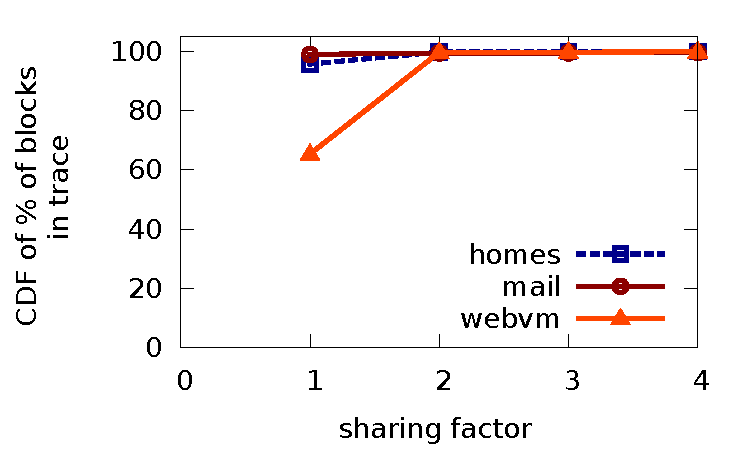
\includegraphics[scale=0.45]{confided-figures/sharing-distrib-from-hashes/reads-writes/cdf-perc-sharing-distrib.pdf}  \hfill
            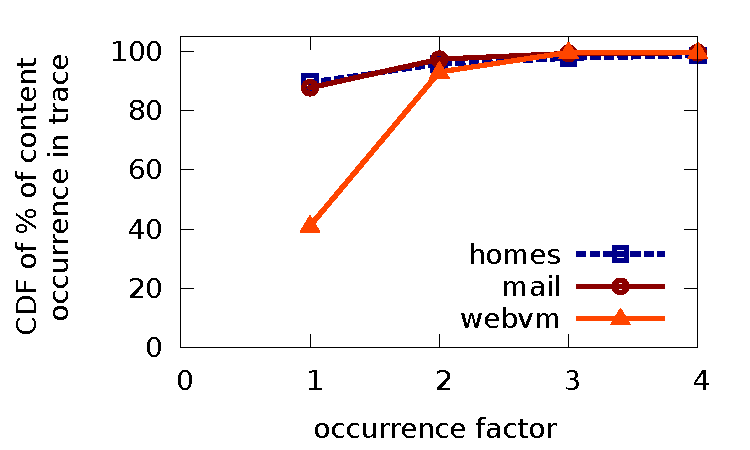
\includegraphics[scale=0.45]{confided-figures/occurrence-distrib/reads-writes/cdf-perc-occurrence-distrib.pdf}
%            \subfloat[\#sharing vs \#occurrence]{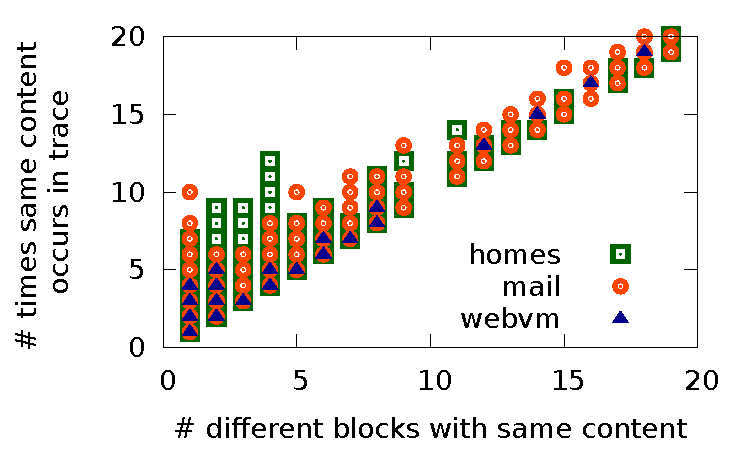
\includegraphics[scale=0.31]{confided-figures/degree-sharing-vs-num-occur-from-hashes/reads-writes/deg-sharing-vs-num-occur.pdf}}
        \vspace{-0.1in}
        \label{fig:similarity-distrib}
        \end{figure}
        \end{columns}
        
        \begin{tikzpicture}[overlay]
            \node[coordinate] (b) at (3.4,2.7) {};
            \node[coordinate] (d) at (3.4,1.9) {};

            \node[coordinate] (f) at (9.6,2.6) {};
            \node[coordinate] (h) at (9.6,1.4) {};

            \begin{scope}
                \pgfsetlinewidth{2pt}
                \draw[<->,style=dotted,color=purple] (d) -- (b) node[midway,right] {35\%};
                \draw[<->,style=dotted,color=purple] (h) -- (f) node[midway,right] {45\%};

            \end{scope}
        \end{tikzpicture}         
        
        %%%%%%%%% BOTTOM-HALF %%%%%%%%%%%
        \vspace{0.1in}
        \begin{block}{Observations}
%         \scriptsize
        \begin{itemize}
            \item \textit{homes} \& \textit{mail} traces have 95\% blocks with sharing factor 1, 
            whereas \textit{webvm} trace has 35\% blocks with sharing factor 2
            \item In \textit{webvm} trace, 45\% content occur twice, compared
                to 6-10\% in \textit{homes} and \textit{mail} traces
%           \item For most pieces of content, occurrence factor $\gt$ sharing factor,

        \end{itemize}
        \end{block}

        \begin{exampleblock}{Conclusions}
%             \footnotesize
            \textit{webvm} trace is likely to benefit
                the most from I/O deduplication
        \end{exampleblock}
    }    
    
    %%%%%%%%%%%%%%%%% SLIDE %%%%%%%%%%%%%%%%%%%%
        \section{Analyzing existing work : IODEDUP}
        \begin{frame}
            \frametitle{Existing\footnote[frame]{Other related work for I/O deduplication \& reduction discussed in report.} I/O deduplication technique: IODEDUP \footnote[frame]{\textit{I/O Deduplication: Utilizing Content Similarity to Improve I/O Performance}}}

        %%%%%%%%% TOP-HALF %%%%%%%%%%%
       \vspace{-0.2in}
        \begin{columns}
            \column{0.5\textwidth}
            \only<1->{
                \hspace{-0.4in}
                \begin{figure}
                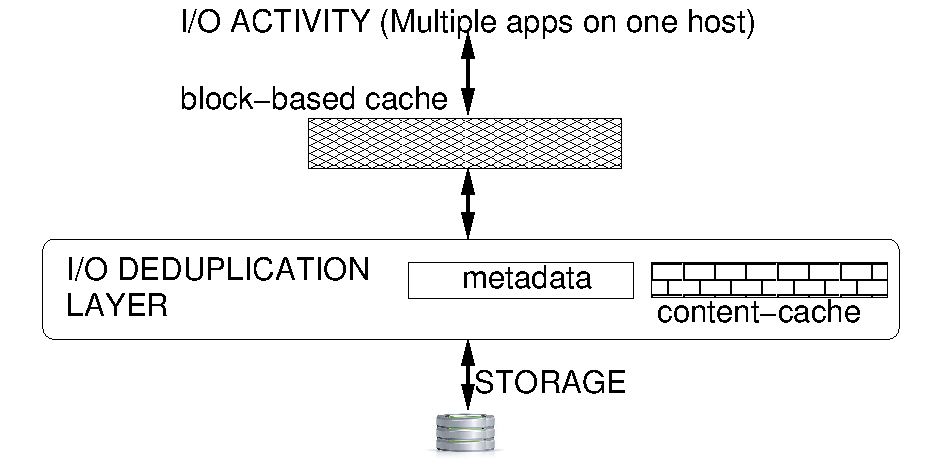
\includegraphics[scale=0.36]{confided-figures/main/sys-arch-iodedup-host.pdf}
                \setbeamerfont{caption name}{size=\scriptsize}
                \setbeamerfont{caption}{size=\scriptsize}
                \vspace{-0.4in}
                \caption{System Architecture of IODEDUP}
                \end{figure}
            }

            \column{0.5\textwidth}
            \only<2->{
                \begin{alertblock}{Drawbacks}
%                     \scriptsize
                \begin{itemize}
                    \item Content-cache \textit{sizing} needs exploration
                    \item Block-cache still faces
                    \textit{duplicate content} problem
                \end{itemize}
                \end{alertblock}
            }
       \end{columns}

        %%%%%%%%% BOTTOM-HALF %%%%%%%%%%%
%        \vspace{-0.1in}
        \begin{columns}
            \column{0.55\textwidth}
            \only<1->{
                \begin{block}{Functioning}
                \begin{itemize}
%                     \scriptsize
                    \item Creates and maintains content-based cache
                    \item Intercepts read requests \& services without
                        accessing disk if possible
                \end{itemize}
                \end{block}
            }
            \column{0.4\textwidth}
            \only<3>{
                \begin{exampleblock}{Our contribution}
                    \begin{itemize}
%                     \scriptsize
                    \item Perform \textit{study of cache
                    effectiveness} for IODEDUP
                    system, using a custom simulator
                    \end{itemize}
                \end{exampleblock}
            }
        \end{columns}

        \end{frame}

    %%%%%%%%%%%%%%%%% SLIDE %%%%%%%%%%%%%%%%%%%%
%   \subsection{Study of cache effectiveness for IODEDUP}
    \begin{frame}
    \frametitle{Study of cache effectiveness for IODEDUP}

        %%%%%%%%% TOP-HALF %%%%%%%%%%%
        \vspace{-0.1in}
        \begin{figure}
        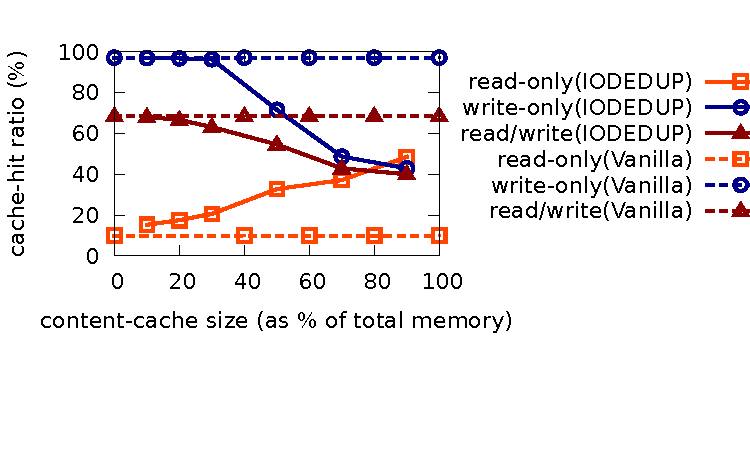
\includegraphics[scale=0.57]{confided-figures/sweetspot-512MB/sweetspot-512MB.pdf}
        \vspace{-0.6in}
        \setbeamerfont{caption name}{size=\small}
        \setbeamerfont{caption}{size=\small}
        \caption{Cache-hit ratios for IODEDUP for \textit{webvm} trace. Total cache 512 MB}
        \end{figure}
       

        %%%%%%%%% BOTTOM-HALF %%%%%%%%%%%
        \begin{block}{Observations}
            \scriptsize
            \begin{enumerate}
                \item Read-only trace has lowest performance at content-cache of 10\% \& highest at 90\%
                \item Write-only performance varies reverse, i.e., highest at 10\% and lowest at 90\%
                \item At content-cache setting of 90\%, read-only performance is 4$\times$ Vanilla, but read/write performance 42\% worse than Vanilla.
            \end{enumerate}
        \end{block}

        \begin{block}{Conclusion: \textcolor{red}{Inconsistence} in achievable cache effectiveness}
%            \scriptsize
%           Depending upon content-cache sizing, the read/write request-mix
%           and the amount of duplicate content, host cache efficiency under
%           the IODEDUP system is inconsistent.         
        \end{block}

    \end{frame}
    %Talk: Above results show non-optimality of IODEDUP. Hence, a more
        % efficient I/O deduplication system is needed. Next, we present
        % our system called DRIVE which performs I/O deduplication via
        % I/O request redirection.

    %%%%%%%%%%%%%%%%% SLIDE %%%%%%%%%%%%%%%%%%%%
    \section{I/O reduction challenges}
    \begin{frame}
        \frametitle{Fundamental issues preventing efficient I/O reduction}

        %can we get a figure here, which shows the three ways in which 
        %I/O reduction is affected.
        %1. using a cache, even block-based reduces I/O
        %2. using a cache in content-dedup fashion reduces more I/O
        %3. deduplicating the content in a cache after I/O is done, reduces I/O toobut to a lesser extent.

        \begin{alertblock}{Issues}
            \begin{enumerate}
                \item In IODEDUP system~\cite{iodedup} has cache inclusiveness problem
                \item Memory deduplication~\cite{satori} works after data is already fetched
                    from disk
            \end{enumerate}
        \end{alertblock}

        \begin{block}{Obvious solution}
        \begin{itemize}
            \item Operate host cache in fully-deduplicated fashion, such
            that only data not present in cache will be fetched from disk
%             thus eliminating the need for separate memory deduplication
%             as well.
        \end{itemize}
        \end{block}
%     \end{frame}

% 
%     %%%%%%%%%%%%%%%%% SLIDE %%%%%%%%%%%%%%%%%%%%
%     \begin{frame}
%         \frametitle{Achieving an approximate-to-Oracle solution}
        \begin{alertblock}{Challenges in implementing obvious solution}
            \begin{enumerate}
                \item Requires change to cache data structures and/or implementation to enable storing of content-based metadata
                \item Requires metadata updates for every cache insertion
                \item Requires invasive monitoring and metadata updates for every eviction from cache
            \end{enumerate}
        \end{alertblock}


    \end{frame}

    %%%%%%%%%%%%%%%%% SLIDE %%%%%%%%%%%%%%%%%%%%
    \section{Our system to achieve I/O reduction : DRIVE}
%   \subsection{System Requirements}
    \frame[shrink]{
    
            \begin{block}{Our Approach}
        \begin{itemize}
            \item Augment the virtual disk driver to \textbf{\textcolor{magenta}{use implicit caching hints}}
            to achieve an approximately fully-deduplicated host cache
        \end{itemize}
        \end{block}
    
    \frametitle{DRIVE: Using implicit caching hints to achieve
        \underline{d}isk I/O \underline{r}eduction \underline{i}n
        \underline{v}irtualized \underline{e}nvironments}

        \only<1->{
        \begin{block}{System Requirements for DRIVE}
%             \textbf{Chunking, hashing, indexing}
        \begin{enumerate}
            \item Intercept block read \textit{request} path for
                \textcolor{magenta}{metadata lookup} and I/O redirection, if present
            \item Intercept block read \textit{return} path for
                \textcolor{magenta}{metadata update}, if not previously present
            \item Intercept block write \textit{request} path for
                \textcolor{magenta}{metadata invalidation}
%            \item (Optionally) Intercept block write \textit{return}
%                path for metadata update.
            \item Maintain \textcolor{magenta}{implicit caching hints} within metadata
                to aid efficient I/O redirection.
        \end{enumerate}
        \end{block}
        }
% 
%         \only<2>{
%             \begin{exampleblock}{Basic difference between DRIVE and IODEDUP}
%             IODEDUP: Services requests using a content-based cache
% 
%             DRIVE: Redirects the I/O requests to duplicate block addresses
%             \end{exampleblock}
%         }
    }
    %Talk: Next, we present the design and implementation of the DRIVE
        % sytem. But before presenting the design, we first present a view
        % placement of the DRIVE module in the virtualization architecture,
        % i.e., at which point does it perform read request interception
        % and redirection.
        
    %%%%%%%%%%%%%%%% SLIDE %%%%%%%%%%%%%%%%%%%%
  \subsection{DRIVE System Design \& Implementation}
    \begin{frame}
    \frametitle{Block request interception-point for DRIVE}

       \vspace{-0.25in}
        \setbeamerfont{caption name}{size=\tiny}
        \setbeamerfont{caption}{size=\tiny}
        \begin{figure}
            \subfloat[KVM split-driver architecture]{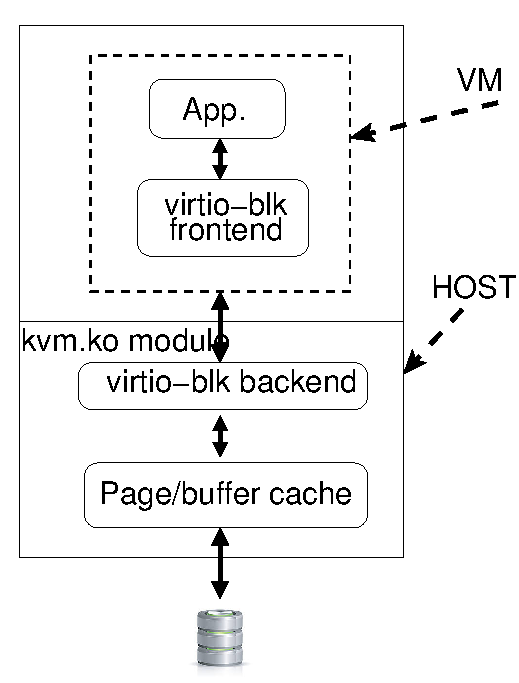
\includegraphics[scale=0.4]{confided-figures/main/kvm-disk-io.pdf}} \hfill
            \subfloat[Xen split-driver architecture]{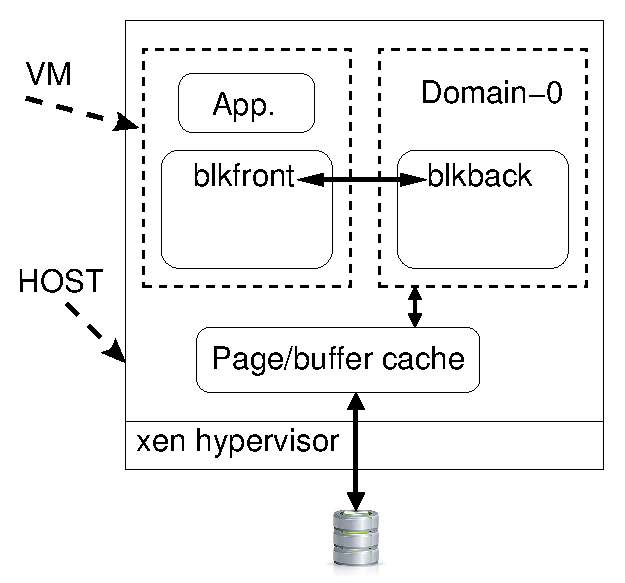
\includegraphics[scale=0.4]{confided-figures/main/xen-disk-io.pdf}}
%           \caption{Split-driver architecture for virtual block devices.}
        \end{figure}
        
        \begin{tikzpicture}[overlay]
            \node[coordinate] (a) at (1.9,3.8) {};
            \node[coordinate] (b) at (5.2,4) {};
            \node[coordinate] (c) at (6.6,4) {};
            \node[coordinate] (d) at (9.6,3.2) {};

            \begin{scope}
                \pgfsetlinewidth{2pt}
                \draw[<-,style=dotted,color=purple] (a) -- (b);
                \draw[->,style=dotted,color=purple] (c) -- (d); %node[midway,right] {45\%};
		\node[rectangle,color=purple] at (6,4.25) {Interception};
		\node[rectangle,color=purple] at (6,3.75) {point};
            \end{scope}
        \end{tikzpicture}             

       \vspace{-0.1in}
        \begin{block}{\scriptsize Interception within VM's front-end driver}
            \scriptsize
            \begin{itemize}
                \item \textcolor{magenta}{De-coupling} of the front-end and back-end
                    drivers enables simple I/O redirection
                \item Results in \textcolor{magenta}{implicit} manipulation of
                    host-cache as a
                    content-deduplicated cache
                \item Exploits individual workload's \textcolor{magenta}{content
                    self-similarity}, useful irrespective of co-hosted VMs
                \item Implementation within generic \texttt{virtio} drivers 
                    \textcolor{magenta}{obviates dependence} on VMM \& guest OS
            \end{itemize}
        \end{block}
    \end{frame}
        
    %%%%%%%%%%%%%%%%% SLIDE %%%%%%%%%%%%%%%%%%%%
    \begin{frame}
    \frametitle{DRIVE metadata store: semantics and usage}

        %%%%%%%%% TOP-HALF %%%%%%%%%%%
      \vspace{-0.15in}
        \begin{columns}
            \column{0.4\textwidth}
                \only<1->{
                \begin{figure}
                    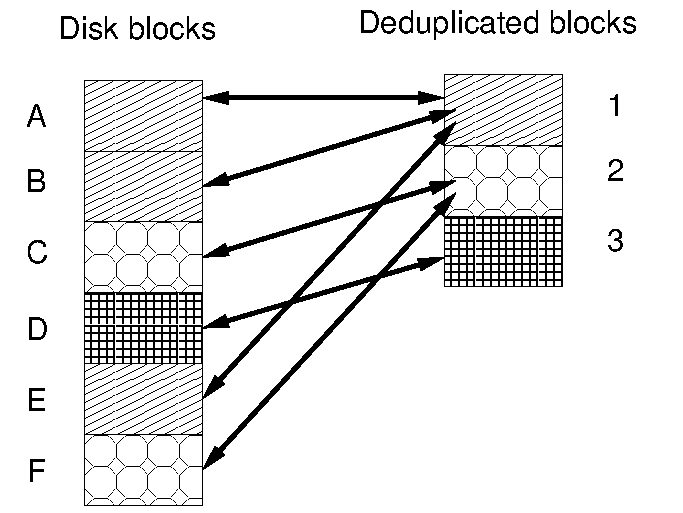
\includegraphics[scale=0.4]{confided-figures/main/deduped-block.pdf}
%                     \vspace{-0.25in}
                    \setbeamerfont{caption name}{size=\scriptsize}
                    \setbeamerfont{caption}{size=\scriptsize}
                    \caption{Semantics of metadata store.}
                \end{figure}
                }

            \column{0.65\textwidth}

            \only<3>{
                \begin{figure}
                            \hspace{-0.4in}
                    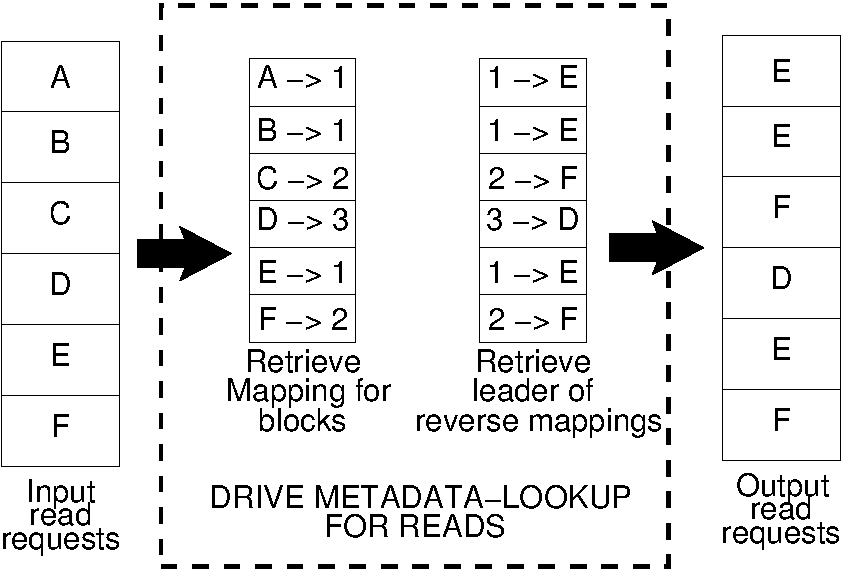
\includegraphics[scale=0.4]{confided-figures/main/dedup-working-reads.pdf}
%                     \vspace{-0.25in}
                    \setbeamerfont{caption name}{size=\scriptsize}
                    \setbeamerfont{caption}{size=\scriptsize}
                    \caption{Example of read request redirection in DRIVE}
                \end{figure}
                }
        \end{columns}
        
        \only<3>{
        \begin{tikzpicture}[overlay]
        \node[rectangle,color=purple] at (11.75,3.25) {cache};
        \node[rectangle,color=purple] at (11.75,2.75) {hits};

        \begin{scope}
        \pgfsetlinewidth{1pt}
            \node[coordinate] (a) at (11.25, 3.25) {};
            \node[coordinate] (b) at (10.25, 4) {};
            \node[coordinate] (c) at (10.25, 2.5) {};
            \node[coordinate] (d) at (10.25, 2) {};

        \pgfsetlinewidth{2pt}
            \draw[->,style=dotted,color=purple] (a) -- (b);
            \draw[->,style=dotted,color=purple] (a) -- (c);
            \draw[->,style=dotted,color=purple] (a) -- (d);

        \end{scope}

        \end{tikzpicture}
        }
        
        %%%%%%%%% BOTTOM-HALF %%%%%%%%%%%
        \only<2->{
        \begin{block}{Obtaining and using hints for I/O redirection}
            \scriptsize
            \begin{enumerate}
                \item When a block is fetched, it is ``known'' to be \textcolor{magenta}{cached}
                \item Above is noted in metadata, \textcolor{magenta}{marked as \textit{leader}}
                \item For next redirection, \textcolor{magenta}{\textit{leader} is used}
            \end{enumerate}
        \end{block}
        }

    \end{frame}
    
    
    %%%%%%%%%%%%%%%%% SLIDE %%%%%%%%%%%%%%%%%%%%
    \begin{frame}
    \frametitle{Evaluating host-cache effectiveness in DRIVE system}
        \vspace{-0.2in}
        \begin{columns}
            \column{0.5\textwidth}
                \begin{figure}
                \hspace{-0.2in}
                    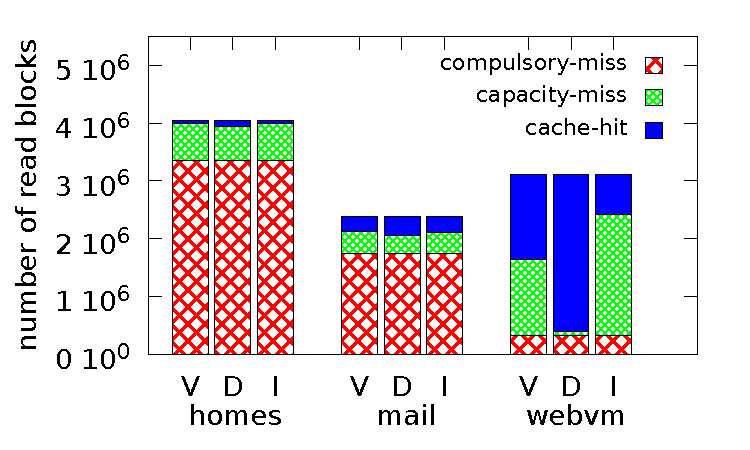
\includegraphics[scale=0.45]{confided-figures/read-response-distrib/reads-writes/read-response-distrib-reads-n-writes.pdf}
        \vspace{-0.2in}
                    \setbeamerfont{caption name}{size=\scriptsize}
                    \setbeamerfont{caption}{size=\scriptsize}
                    \caption{Classification of read responses}
                \end{figure}

            \column{0.5\textwidth}
                \begin{figure}
		    \hspace{-0.35in}
                    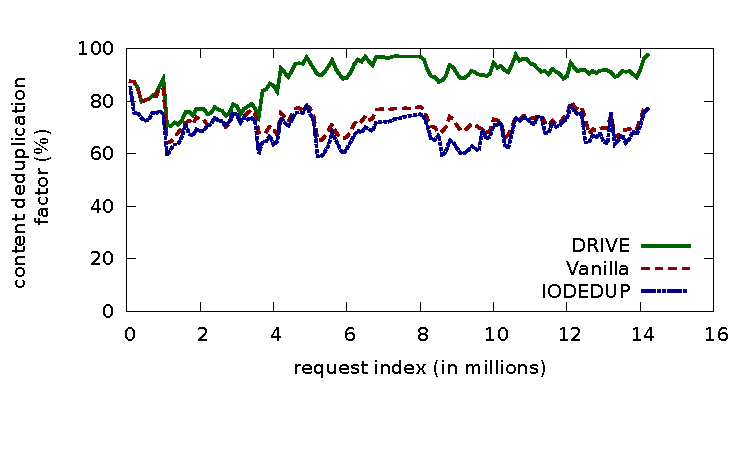
\includegraphics[scale=0.53]{confided-figures/contentdedup-factor/contentdedupfactor.pdf}
        \vspace{-0.3in}
                    \setbeamerfont{caption name}{size=\scriptsize}
                    \setbeamerfont{caption}{size=\scriptsize}
                    \caption{Content deduplication factor of page cache upon \textit{webvm} trace.}
                \end{figure}
        \end{columns}

        \begin{exampleblock}{Conclusions}
            \scriptsize
            \begin{itemize}
                \item Both \textit{homes} and \textit{mail} workloads have huge number of compulsory misses, whereas the \textit{webvm} workload has significantly fewer.
                \item DRIVE \textcolor{magenta}{decreases number of capacity misses to 5\%} of Vanilla
                \item DRIVE achieves up to \textcolor{magenta}{97\% deduplication} in block-cache
            \end{itemize}
        \end{exampleblock}
    \end{frame}

    %%%%%%%%%%%%%%%%% SLIDE %%%%%%%%%%%%%%%%%%%%
    \begin{frame}
    \frametitle{Identifying similarity in multiple virtual machines}

        \vspace{-0.2in}
        \begin{columns}
            \column{0.6\textwidth}
                \begin{figure}
                    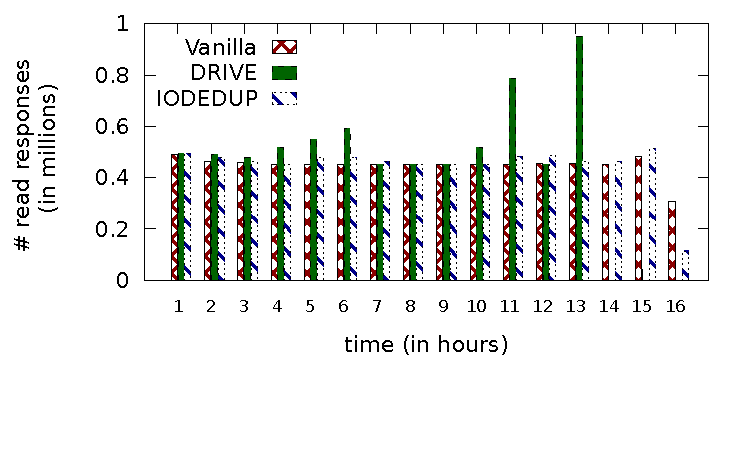
\includegraphics[scale=0.55]{confided-figures/aggregate-hw-replay/reads-writes/timeseriesperf-hour.pdf}
                    \vspace{-0.65in}
                    \setbeamerfont{caption name}{size=\scriptsize}
                    \setbeamerfont{caption}{size=\scriptsize}
                    \caption{Read response throughput for aggregated (\textit{homes}+\textit{webvm}) trace.}
                \end{figure}

                \renewcommand{\tabcolsep}{1pt}
                \vspace{-0.4in}
                \begin{table}
                \caption{Performance for aggregated trace replay}
                \scriptsize
                    \begin{tabular}{|c|c|c|c|} \hline               
                    \textbf{Scheme} & \textbf{Cache-hit} & \textbf{Disk reads} & \textbf{Avg. read}  \\
                    \textbf{} & \textbf{ratio (\%)} & \textbf{reduced(\%)} & \textbf{response latency}  \\ 
                    \textbf{} &  &  & \textbf{(msec)}  \\ \hline
                    %\textbf{} & \textbf{} & \textbf{} & \textbf{latency} \\ \hline
                    Vanilla & 61.2 & 1.6 & 7.9 \\ \hline
                    \rowcolor{green} DRIVE & 67.6 & 18.5 & 6.5 \\ \hline
                    IODEDUP & 62.4 & 4.3  & 7.7 \\ \hline
                    \end{tabular}
                    \setbeamerfont{caption name}{size=\scriptsize}
                    \setbeamerfont{caption}{size=\scriptsize}
                    
                %\vspace{-0.15in}
                \end{table}

            \column{0.4\textwidth}
            \begin{exampleblock}{Conclusions}
            \scriptsize
                \begin{itemize}
                    \item DRIVE completes earlier due to higher number of
                        responses per hour on average\footnote[frame]{Throughput derived from measured cache-hits \& disk-reads and assumed latency values.}.
                    \vspace{0.2in}
                    \item Huge margin in percentage of disk reads reduced
                \end{itemize}
            \end{exampleblock}
            
            \begin{block}{Summary of DRIVE}
		\scriptsize
		\begin{enumerate}
		 \item Performs implicit caching hint-based I/O redirection
		 \item Simulation-based evaluation shows promise---up to 97\% content-deduplicated cache achieved
		 \item Further analysis requires more production traces
		\end{enumerate}

            \end{block}


        \end{columns}
    \end{frame}    
        
    %%%%%%%%%%%%% SLIDE %%%%%%%%%%%%%%
    \begin{frame}
	\frametitle{Dataset survey for I/O deduplication traces}
	
	\vspace{-0.1in}
	\begin{block}{}
	    \textcolor{magenta}{To find for other public datasets that can be used for our evaluation}
	\end{block}
	
	\vspace{-0.1in}
\begin{figure}
	\centering
	\subfloat[Conference-name tag cloud]{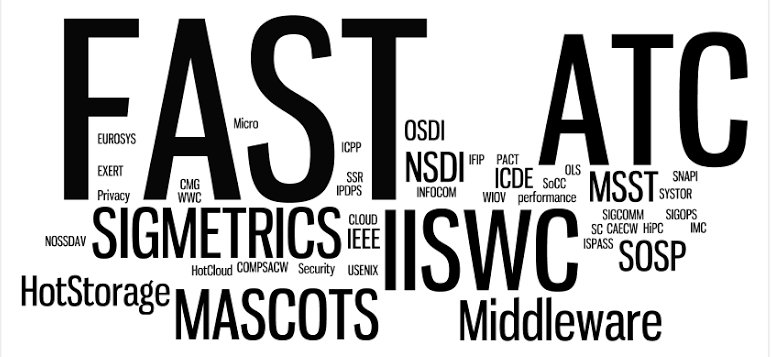
\includegraphics[scale=0.13]{presyn-figures/conference-names-wordle.jpg}} ~~~~~~~~~~~
	\subfloat[Year-of-publication tag cloud]{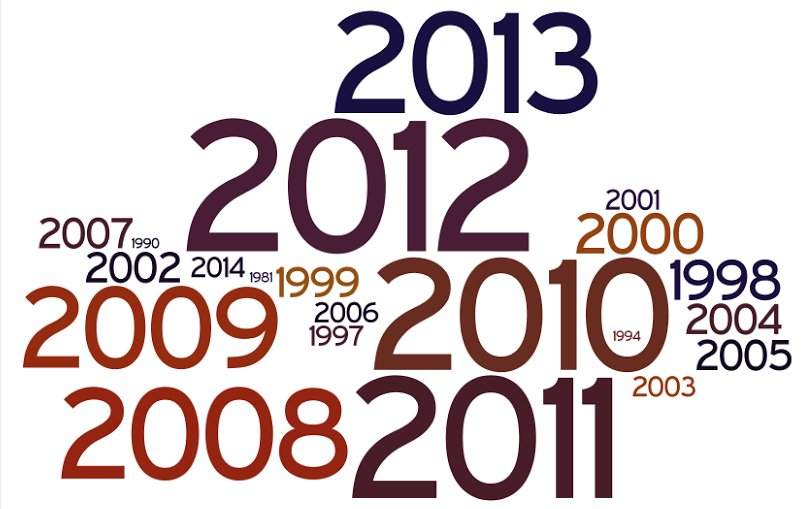
\includegraphics[scale=0.13]{presyn-figures/year-of-publication-wordle.jpg}}	
% 	\caption{Representation of the conferences and the years of publication covered in our survey}
	\label{fig:tag-clouds}
\end{figure}

      \begin{block}{Three types of workloads used in literature}
	\begin{enumerate}
	 \item Synthetic benchmarks
	 \item Production I/O traces
	 \item Production filesystem datasets
	\end{enumerate}
      \end{block}

      \begin{alertblock}{Our requirement}
	  I/O traces having content representation as well---not available publicly.
      \end{alertblock}

    \end{frame}

    %%%%%%%%%%%%% SLIDE %%%%%%%%%%%%%%
    \begin{frame}
	\frametitle{Literature survey for ``realistic'' dataset generation}
	
	\vspace{-0.1in}
	\begin{block}{Types of datasets generated}
	 \begin{enumerate}
	  \item I/O traces (without content)~\cite{storagecharacterization, storagereplay, storagemodeling, flexi-replay, jump-based-synthetic}
% 	  \item Network traces (without content)~\cite{echo}
	  \item Filesystem content (without I/O traces)~\cite{generating-datasets}
	 \end{enumerate}
	\end{block}

	\begin{block}{Relevant characteristics for I/O traces\footnote[frame]{\textit{webvm} and \textit{homes} trace characterization presented in report.}}
% 	 \begin{itemize}
	    \textcolor{magenta}{Block accessed distribution} \& \textcolor{magenta}{Jump distances}---\textit{spatial locality} \\
	    \textcolor{magenta}{Run lengths} \& \textcolor{magenta}{Block reuse distances}---\textit{temporal locality}
% 	 \end{itemize}

	\end{block}

	\begin{block}{General approach}
	  \begin{enumerate}
	   \item Capture Multi-dimensional distributions and/or Markov models
	   \item Use above captured models to create new traces with similar properties
	   \item Vary appropriate parameters to create different traces as necessary
	  \end{enumerate}

	\end{block}	
	
    \end{frame}


    %%%%%%%%%%%% SLIDE %%%%%%%%%%%%%%
    \begin{frame}{}
	\frametitle{Content-defined characterization of \textit{webvm} trace}
	\vspace{-0.23in}
        \begin{columns}
            \begin{column}{0.5\textwidth}
	      \begin{figure}
		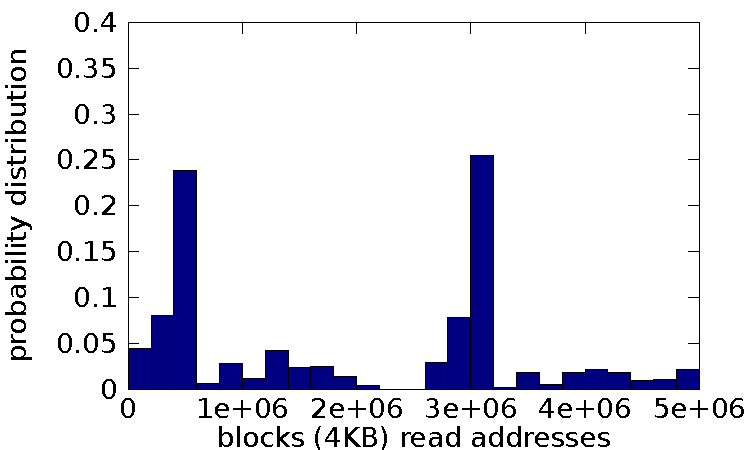
\includegraphics[scale=0.36]{tracechar-figures/21-day/webvm-block-read-appended-21-prob-40perc.pdf}
		\vspace{-0.15in}
		\caption{Block access distribution}
	      \end{figure}
            \end{column}
            \begin{column}{0.5\textwidth}
	      \begin{figure}
		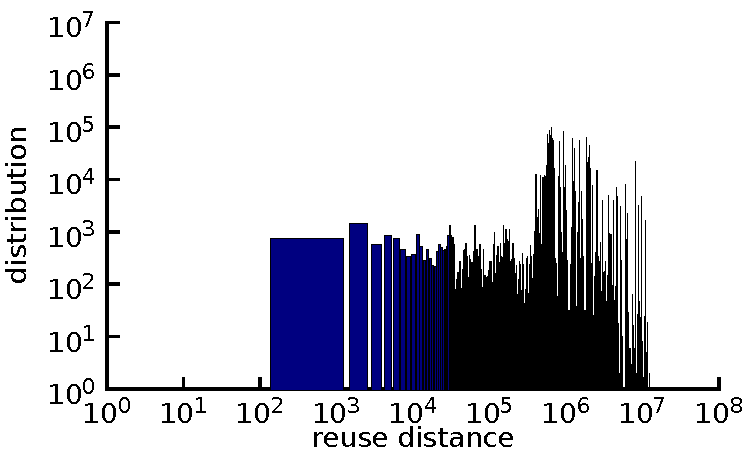
\includegraphics[scale=0.36]{tracechar-figures/21-day/webvm-reuse-dist-distrib-readonly-appended-21-loglog.pdf}
		\vspace{-0.15in}
		\caption{Block reuse distribution}		
	      \end{figure}             
            \end{column}
	\end{columns}

	\vspace{-0.25in}	
        \begin{columns}
            \begin{column}{0.5\textwidth}
	      \begin{figure}
		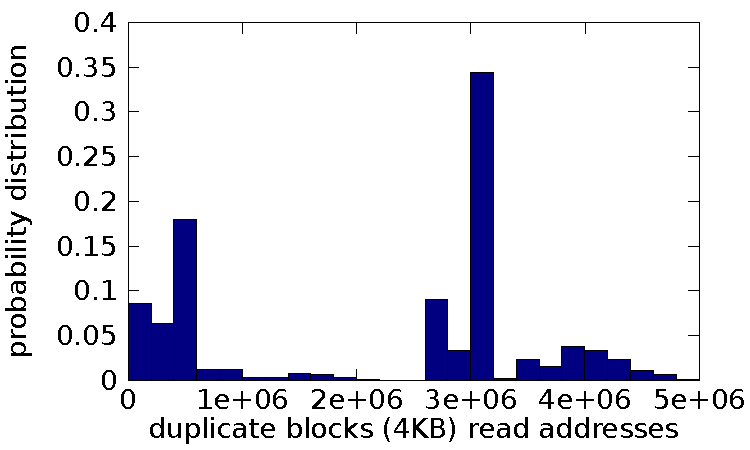
\includegraphics[scale=0.36]{tracechar-figures/21-day/webvm-dedup-block-read-appended-21-prob-40perc.pdf}
		\vspace{-0.15in}
		\caption{Duplicate block access distrib}		
	      \end{figure}             
            \end{column}
            \begin{column}{0.5\textwidth}
	      \begin{figure}
		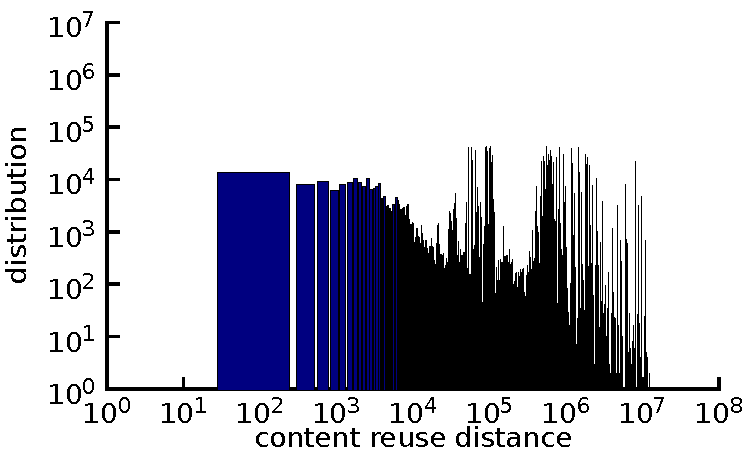
\includegraphics[scale=0.36]{tracechar-figures/21-day/webvm-reuse-dist-distrib-dedup-readonly-appended-21-loglog.pdf}
		\vspace{-0.15in}
		\caption{Content reuse distribution}		
	      \end{figure}             
            \end{column}
	\end{columns}     

	\vspace{-0.1in}
    \begin{exampleblock}{Observations}
    \scriptsize
     \begin{itemize}
      \item Even duplicate content access has \textcolor{magenta}{spatial locality} property
      \item \textcolor{magenta}{Temporal locality} is higher for content than block
     \end{itemize}

    \end{exampleblock}	
 
 \end{frame}    
        
    %%%%%%%%%%%%% SLIDE %%%%%%%%%%%%%%
    \section{Conclusions}
    \frame{
        \frametitle{DRIVE system summary \& conclusions}

        \begin{exampleblock}{}
        \begin{itemize}
%             \scriptsize
            \item In this component, we addressed I/O reduction via deduplication
                \vspace{0.1in}
            \item We analyzed existing work (IODEDUP) and showed that its
                performance is inconsistent depending on the read/write request-mix
                of the workload.
                \vspace{0.1in}
            \item We presented design \& implementation of our DRIVE system
                \vspace{0.1in}
            \item Simulation evaluation shows promise---achieves 97\% content
                deduplication of the host cache.
            \item We concluded with a survey of publicly available datasets, as
		  well as benchmark generation literature, to make the case that
		  future work towards I/O deduplication benchmarks is necessary
        \end{itemize}
        \end{exampleblock}

% 
%     \vspace{0.3in}
%     \begin{exampleblock}{}
%         \footnotesize
%     Systems and Networking Research Group (SynerG), IIT Bombay @
%     \url{http://www.cse.iitb.ac.in/synerg}
%     \end{exampleblock}

    }        
    
% %%%%%%%%%%%%%%%%%%%%%% BACKUP SLIDES BEGIN $$$$$$$$$$$$$$$$$$$$$$$$$$$$$$$$$$$$$$$$$$$$    
\backupbegin
%%%%%%%%%%%%%%%%%%%%%%%% BIBLIOGRAPHY %%%%%%%%%%%%%%%%%%%%%%%%
    \begin{frame}[allowframebreaks]
        \frametitle{Bibliography}
\bibliographystyle{unsrt}
\tiny\bibliography{defense}
    \end{frame}

%     %%%%%%%%%%%%%%%%%% SLIDE %%%%%%%%%%%%%%%%%%%%
%     \frame{
%         \textcolor{blue}{Questions/Comments?}
%     }
% 
%     %%%%%%%%%%%%%%%%%% SLIDE %%%%%%%%%%%%%%%%%%%%
%     \frame{
%         \textcolor{blue}{BACKUP SLIDES}
%     }
% 
%     %%%%%%%%%%%%%%%%%% SLIDE %%%%%%%%%%%%%%%%%
% %%%%%%%%%%%%% SLIDE %%%%%%%%%%%%%%
%     \section{Benchmarking the Effect of Colocation on CPU Usage}
%     \subsection{Benchmarking: Setup and Tools}
%     \frame[shrink]{
%         \frametitle{Benchmarking: Setup and Tools}
%         %setup picture and the tools used in dom0 and domU
%         \begin{columns}
%             \column{0.65\textwidth}
% \noindent\makebox[\textwidth]{%  check this SSS........
% \begin{tabular}{c}
% % \begin{figure}
% % \centering
% % 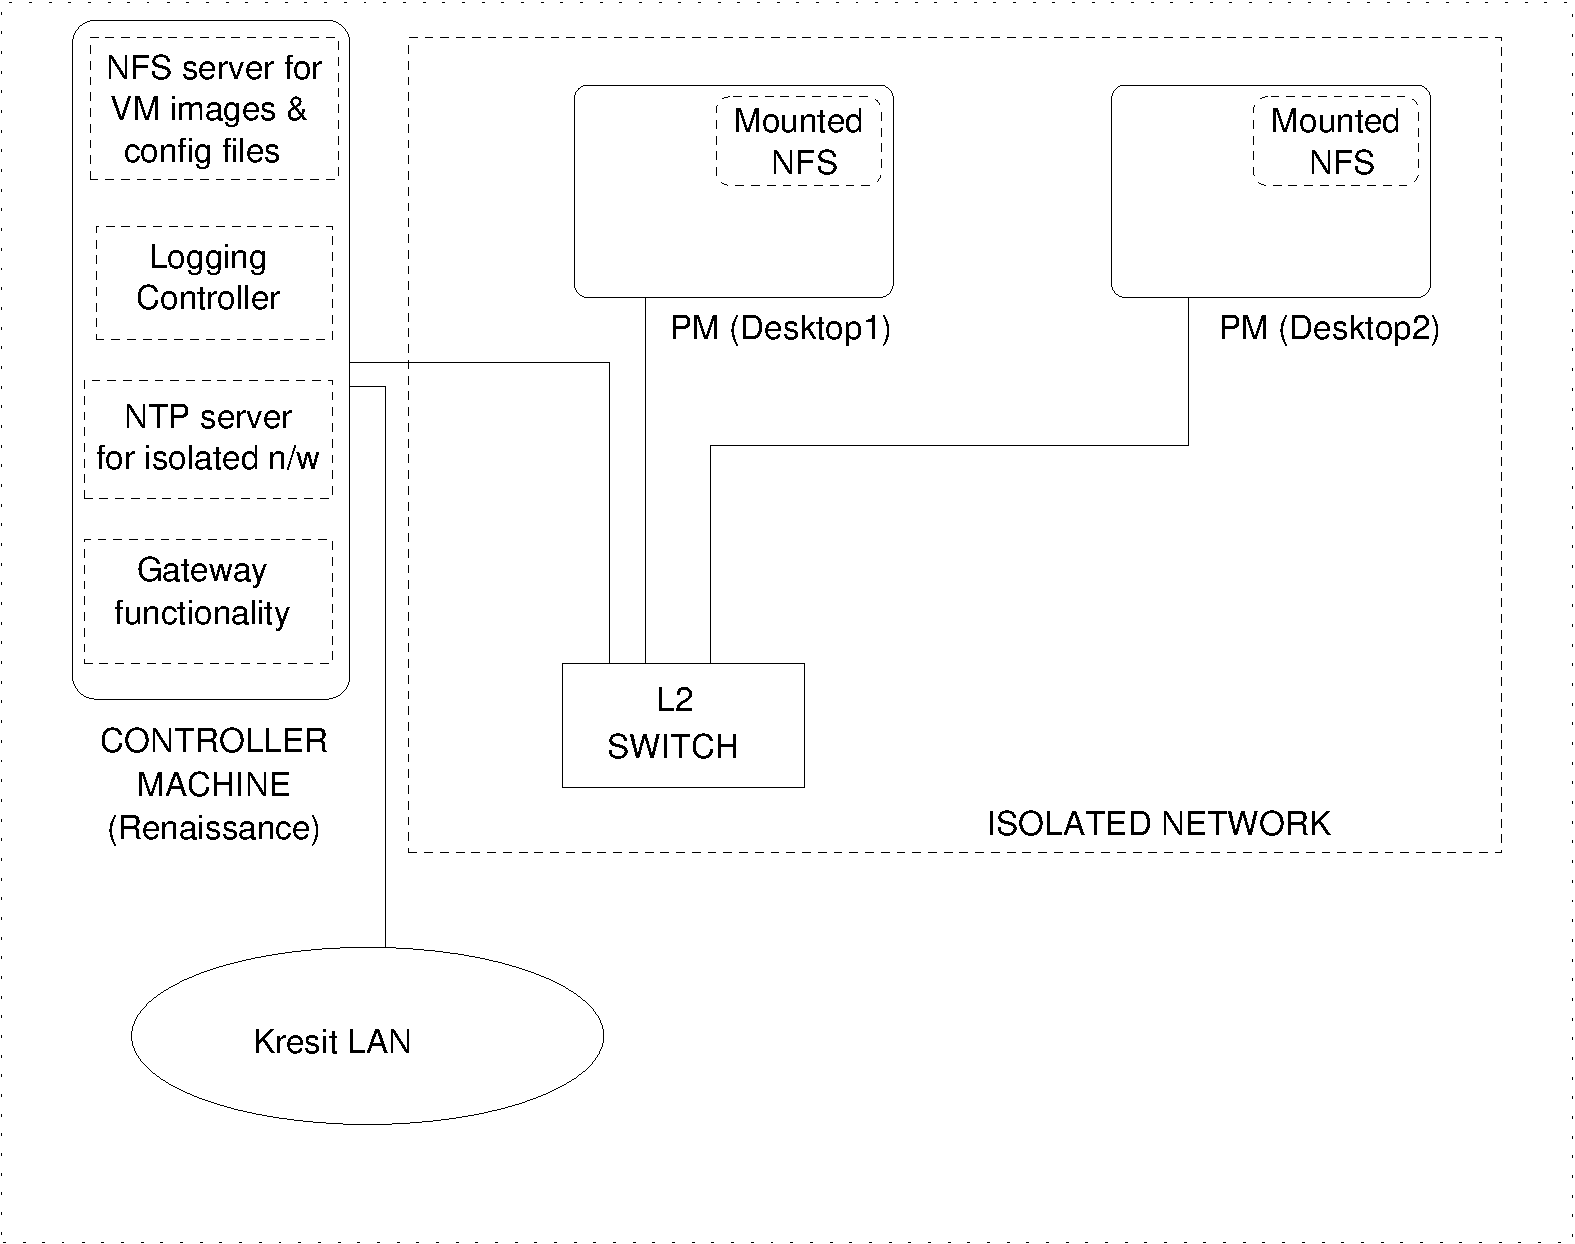
\includegraphics[scale=0.35]{figures/setup-for-profiling.pdf}
% 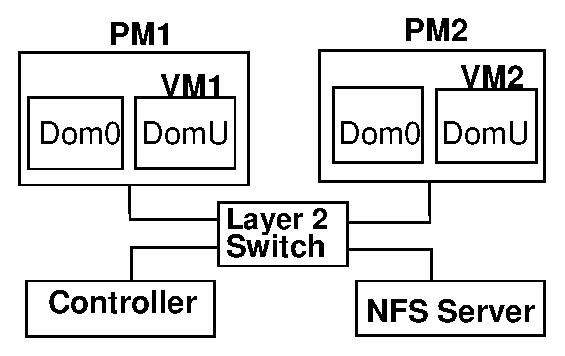
\includegraphics[width=2.6in]{jss-figures/benchmark.eps}
% % \caption{Isolated setup for benchmarking, profiling and model evaluation.}
% % \label{setup-for-profiling}
% % \end{figure}
% \end{tabular}
% }
%         \begin{block}{Microbenchmarks}
%          \begin{itemize}
%           \item {\color {BrightForestGreen}CPU}: $10\%$ to $90\%$, steps of $10\%$
%         \item {\color {BrightForestGreen}Network}: $10$Mbps to $90$Mbps, steps of $10$Mbps
%         \item {\color {BrightForestGreen}Disk}: $0$ - $1500$ blocks/sec, powers of $2$
%          \end{itemize}
%         \end{block}
% 
% %           \pause
%             \column{0.35\textwidth}
%             \begin{block}{Expt. scenarios}
%              \begin{itemize}
%               \item Dispersed VMs
%               \item Colocated VMs
%              \end{itemize}
%             \end{block}
% 
%             \begin{block}{Dom0 Measurement Tools}
%              \begin{itemize}
%               \item xentop
% %           \item Xenmon
%             \item sar
% %           \item libpcap
% %           \item Top
%              \end{itemize}
% 
%             \end{block}
%             \begin{block}{DomU Measurement Tools}
% %             Sar
%              \begin{itemize}
%               \item tcpdump
%               \item sar
% %           \item Top 
%              \end{itemize}
% 
%             \end{block}
% 
% %           \pause
%         \end{columns}
%     }
%     
%     \begin{frame}
%      \frametitle{Effect of Colocation for Other Workloads}
% \begin{table}
% \centering
% % \noindent\makebox[\textwidth]{% 
% \begin{tabular}{|c|c|c|} \hline
% \textbf{Non-affine} & \multicolumn{2}{|c|}{\textbf{Percentage CPU utilization}} \\ \cline{2-3} \cline{2-3}
% \textbf{Receive} & \textbf{Dispersed case} & \textbf{Colocated case} \\
% (Mbps) & $VM_1,VM_2, \sum Dom0_i$ & $VM_1,VM_2,Dom0$ \\ \hline
% % $<$20, 10$>$ & 3, 2, 12 & 3, 2, ~8 \\ \hline
% % $<$20, 30$>$ & 4, 5, 14 & 3, 5, 11 \\ \hline
% $<$20, 50$>$ & 4, 7, 18 & 4, 7, 14 \\ \hline
% $<$20, 70$>$ & 4, 9, 21 & 4, 9, 17 \\ \hline
% $<$40, 10$>$ & 6, 2, 15 & 6, 2, 11 \\ \hline
% $<$40, 30$>$ & 7, 5, 18 & 7, 5, 15 \\ \hline
% $<$40, 50$>$ & 7, 7, 21 & 7, 7, 18 \\ \hline
% $<$60, 10$>$ & 8, 2, 18 & 8, 2, 14 \\ \hline
% % $<$60, 30$>$ & 8, 5, 21 & 8, 5, 18 \\ \hline
% \end{tabular}
% % }
% \caption{Percentage CPU usage for non-affine Rx.}
% %\caption{Non-affine receive benchmarking results for colocated provisioning}
% \label{nonaff-rx-benchmark}
% \vspace{-0.3in}
% \end{table}
% 
%     \begin{block}{}
%      Similar observations for other workloads - disk read/write and CPU
%     \end{block}
%     \end{frame}
% 
%     %%%%%%%%%%%% SLIDE
%     \frame{
%         \frametitle{Evaluation using RUBiS Benchmark: Results}
% \vspace{-0.2in}
% %       \noindent\makebox[\textwidth]{% check this SSS........
%          \begin{columns}
%             \column{0.5\textwidth}
%                 \begin{figure}
%                 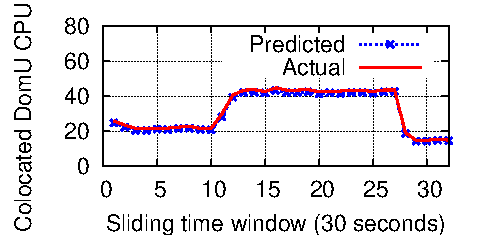
\includegraphics[scale=0.65]{figures/rubis-co-domu1.pdf}\caption{Web tier}
%                 \end{figure}
% %               \pause
%             \column{0.5\textwidth}
%                 \begin{figure}
%                 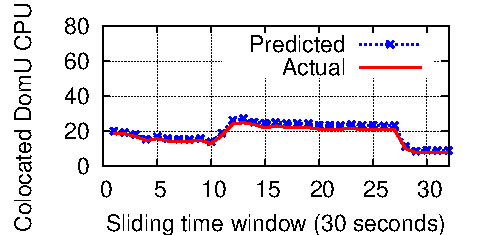
\includegraphics[scale=0.65]{figures/rubis-co-domu2.pdf}\caption{DB tier}
%                 \end{figure}
%          \end{columns}
% % }
% 
%         \noindent\makebox[\textwidth]{% check this SSS........
%          \begin{columns}
%             \column{0.5\textwidth}
%                 \begin{figure}
%                 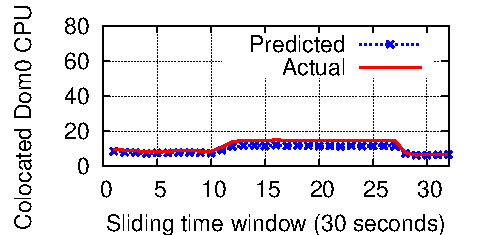
\includegraphics[scale=0.65]{figures/rubis-co-dom0.pdf}\caption{Dom0}
%                 \end{figure}
%             \column{0.5\textwidth}
%                 \begin{exampleblock}{Conclusions}
%                 \begin{itemize}
%                 \item $90^{th}$ percentile error of 3\% absolute CPU for colocation model.
%                   \item Similar observations for dispersion model also.
%                 \end{itemize}
% 
% 
%                 \end{exampleblock}
%         \end{columns}
% }
%     }    
%     
%     %%%%%%%%%%%% SLIDE
%     \frame{
%         \frametitle{RUBiS Benchmark Results: Reverse Model}
% \vspace{-0.2in}
% %       \noindent\makebox[\textwidth]{% check this SSS........
%          \begin{columns}
%             \column{0.5\textwidth}
%                 \begin{figure}
%                 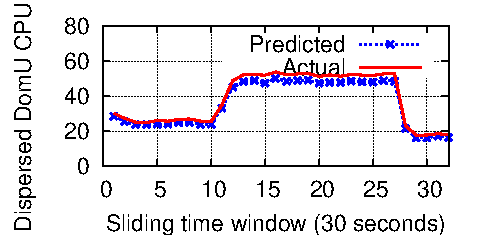
\includegraphics[scale=0.65]{figures/rubis-dis-domu1.pdf}\caption{Web tier}
%                 \end{figure}
% %               \pause
%             \column{0.5\textwidth}
%                 \begin{figure}
%                 \includegraphics[scale=0.65]{figures/rubis-dis-domu2.pdf}\caption{DB tier}
%                 \end{figure}
%          \end{columns}
% % }
% 
%         \noindent\makebox[\textwidth]{% check this SSS........
%          \begin{columns}
%             \column{0.5\textwidth}
%                 \begin{figure}
%                 \includegraphics[scale=0.65]{figures/rubis-dis-dom01.pdf}\caption{Dom0 of Web tier}
%                 \end{figure}
%             \column{0.5\textwidth}
%                 \begin{figure}
%                 \includegraphics[scale=0.65]{figures/rubis-dis-dom02.pdf}\caption{Dom0 of DB tier}
%                 \end{figure}
%         \end{columns}
% 	 }
%     }
%     
%     %%%%%%%%%%%%%%%%% SLIDE %%%%%%%%%%%%%%%%%%%%
%     \section{Experimental evaluation}
%     \begin{frame}
%     \frametitle{Evaluation using custom simulator (1GB cache)}
% 
%         \vspace{-0.4in}
%         \begin{columns}
%             \column{1\textwidth}
%             \setbeamerfont{caption name}{size=\scriptsize}
%             \setbeamerfont{caption}{size=\scriptsize}
%                 \begin{figure}
%                     \subfloat[Cache-hit performance]{\includegraphics[scale=0.4]{confided-figures/cache-hit-rate/reads-writes/eval-reads-n-writes.pdf}}
%                     \subfloat[Disk read reduction]{\includegraphics[scale=0.4]{confided-figures/disk-fetches-averted/reads-writes/readsaverted-reads-n-writes.pdf}}
%                     
%                     \subfloat[Read response latency]{\includegraphics[scale=0.4]{confided-figures/io-latency-normal/reads-writes/iolatency-reads-n-writes.pdf}}
%                     \subfloat[Read response throughput]{\includegraphics[scale=0.4]{confided-figures/io-latency-normal/reads-writes/iothroughput-reads-n-writes.pdf}}
%                 \end{figure}
% %       \footnotetext[7]{Disk read latency 8ms \& cache read latency 
% %           230ns assumed~\cite{gustavo-blogpost}}
% 
% % 
% %             \column{0.2\textwidth}
% %                 \vspace{0.1in}
% %                 \setbeamerfont{block title}{size=\tiny}
% %                 \setbeamerfont{block body}{size=\tiny}
% %                 \begin{block}{Measured metrics}
% %                     (a) Cache-hits \\ (b) Disk reads
% %                 \end{block}
% % 
% %                 \begin{block}{Derived metrics\footnote[frame]{Average disk-read latency 8ms \& cache-read latency 230ns assumed~\cite{gustavo-blogpost}.}}
% %                     (c) Response latency \\ (d) throughput
% %                 \end{block}
% % 
% %                 \setbeamerfont{example block title}{size=\tiny}
% %                 \setbeamerfont{example block body}{size=\tiny}
% %                 \begin{exampleblock}{Conclusions}
% %                 \tiny
% %                 \begin{itemize}
% %                     \item DRIVE has higher cache-hit ratios \& disk reads reduced
% % %                   \item For disk reads reduced, DRIVE has nearly 85\% improvement over Vanilla, and a 2.8$\times$ improvement over IODEDUP
% %                     \item DRIVE has lower average read response time \& higher read response throughput
% %                 \end{itemize}
% %                 \end{exampleblock}
% 
%         \end{columns}
%         
%                 \begin{exampleblock}{Conclusions}
%                 \scriptsize
%                     DRIVE has higher cache-hit ratios \& disk reads reduced
% %                   \item For disk reads reduced, DRIVE has nearly 85\% improvement over Vanilla, and a 2.8$\times$ improvement over IODEDUP
% %                     \item DRIVE has lower average read response time \& higher read response throughput
%                 \end{exampleblock}
% 
%     \end{frame}

%     
%     %%%%%%%%%%%%%%%%% SLIDE %%%%%%%%%%%%%%%%%%%%
%     \begin{frame}
%     \frametitle{CPU overhead details: Write-flow \& Read-flow}
% 
%         \begin{columns}
%             \column{0.5\textwidth}
%                 \begin{figure}
%                     \includegraphics[scale=0.30]{confided-figures/main/dedup-working-writeflow.pdf}
%                     \setbeamerfont{caption name}{size=\tiny}
%                     \setbeamerfont{caption}{size=\tiny}
%                     \caption{Flow path(s) for write requests: \textit{The
%                         differences due to
%                         cache mode (write-back, write-through) and
%                         metadata update mode for writes (updated, not-updated)
%                         are indicated.}}
%                 %    \vspace{-0.25in}
%                 \end{figure}
% 
%             \column{0.5\textwidth}
%                 \begin{figure}
%                     \includegraphics[scale=0.30]{confided-figures/main/dedup-working-readflowcomp.pdf}
%                     \setbeamerfont{caption name}{size=\tiny}
%                     \setbeamerfont{caption}{size=\tiny}
%                     \caption{Flow path(s) for read requests: \textit{P is requested block ID and Q is corresponding leader block ID.}}
%                 \end{figure}
% 
%         \end{columns}
%     \end{frame}
% 
% 
%     %%%%%%%%%%%%%%%%% SLIDE %%%%%%%%%%%%%%%%%%%%
%     \frame[shrink]{
%     \frametitle{Effect of metadata updates during writes}
% 
% %\renewcommand{\tabcolsep}{1pt}
% \begin{table}
% \small
% \caption{Latency parameters used for evaluation}
% \begin{tabular}{|c|l|c|} \hline
% \textbf{Sr. No.} & \textbf{Component} & Latency \\ \hline
% 1 & \textit{Block-cache lookup} & 83ns \\
% 2 & \textit{Block-cache update} & 83ns \\
% \rowcolor{Gray} 3 & \textit{Metadata lookup} & 100ns \\
% \rowcolor{Gray} 4 & \textit{Content-cache lookup} & 100ns \\
% \rowcolor{Gray} 5 & \textit{Metadata update} & 100ns \\
% \rowcolor{Gray} 6 & \textit{Content-cache update} & 100ns \\
% \rowcolor{Gray} 7 & \textit{Metadata invalidate} & 100ns \\
% 8 & \textit{Disk read} & 13.7ms \\
% 9 & \textit{Disk write (write-back)} & 83ns \\
% 10 & \textit{Disk write (write-through)} & 15ms \\ \hline
% \end{tabular}
% %\vspace{-0.15in}
% \end{table}
% 
% %\renewcommand{\tabcolsep}{1pt}
% \begin{table}
% \small
% \caption{Write-path latency with metadata-updated (MeU) and not updated (MeNU)}
% \label{tab:writepath-list}
% \centering
% \begin{tabular}{|l|c|c|c|c|} \hline
% \textbf{Write-through} & \textbf{System} & \textbf{Metadata} & \textbf{Latency} & \textbf{Throughput} \\
% \textbf{or Write-back} & & \textbf{Update?}  & \textbf{per request} & \textbf{(million per hour)} \\ \hline
% Write-through & Vanilla & - & $\sim$15ms & 0.216 \\
% Write-through & DRIVE & MeU & $\sim$15ms & 0.216 \\
% Write-through & DRIVE & MeNU & $\sim$15ms & 0.216 \\
% Write-through & IODEDUP & - & $\sim$15ms & 0.216 \\ \hline
% Write-back & Vanilla & - & 100ns & 36000 \\
% \rowcolor{red} Write-back & DRIVE & MeU & $\sim$33.33us & 108 \\
% Write-back & DRIVE & MeNU & 200ns & 18000 \\
% Write-back & IODEDUP & - & 100ns & 36000 \\ \hline
% \end{tabular}
% %\vspace{-0.15in}
% \end{table}
%     }
% 
%     %%%%%%%%%%%%%%%%% SLIDE %%%%%%%%%%%%%%%%%%%%
%     \frame[shrink]{
%     \frametitle{Exploring read-path scenarios in more detail}
% \renewcommand{\tabcolsep}{1pt}
% \begin{table}
% \small
% \caption{With metadata-updated upon writes (MeU)}
% \begin{tabular}{|l|c|c|c|c|c|c|c|c|c|} \hline
%  & \multicolumn{2}{c|}{\textbf{Vanilla}} & \multicolumn{3}{c|}{\textbf{DRIVE (with MeU)}} & \multicolumn{4}{c|}{\textbf{IODEDUP (with MeU)}}  \\ \cline{2-10}
%  & & & \texttt{cacheR} & \multicolumn{2}{c|}{\texttt{diskR}} & \multicolumn{2}{c|}{\texttt{cacheR}} & \multicolumn{2}{c|}{\texttt{diskR}} \\ \cline{4-10}
%  & & & \texttt{block} & \texttt{metadata} & \texttt{block} & \texttt{block} & \texttt{content} & \texttt{metadata} & \texttt{content} \\
% \textbf{Step} & \texttt{cacheR} & \texttt{diskR} & \texttt{hit} & \texttt{miss} & \texttt{miss} & \texttt{hit} & \texttt{hit} & \texttt{miss} & \texttt{miss} \\ \hline
% \rowcolor{Gray} \textit{Metadata lookup} & & & \ding{51} & \ding{51} & \ding{51} & & \ding{51} &\ding{51} & \ding{51} \\
% \textit{Block-cache lookup} & \ding{51} & \ding{51} & \ding{51} & \ding{51} & \ding{51} & \ding{51} & \ding{51} & \ding{51} & \ding{51} \\
% \rowcolor{Gray} \textit{Content-cache lookup} & & & & & & & \ding{51} & & \ding{51} \\
% \textit{Disk read} & & \ding{51} & & \ding{51} & \ding{51} & & & \ding{51} & \ding{51}  \\
% \textit{Block-cache update} & & \ding{51} & & \ding{51} & \ding{51} & & \ding{51} & \ding{51} & \ding{51} \\
% \rowcolor{Gray} \textit{Metadata update} & & & & \ding{51} & & & & \ding{51} & \\
% \rowcolor{Gray} \textit{Content-cache update} & & & & & & & & \ding{51} & \ding{51} \\ \hline \hline
% \rowcolor{green} \textit{Total read latency} & 83ns &$\sim$13.7ms & \textcolor{red}{183ns} & $\sim$13.7ms & $\sim$13.7ms & 83ns & \textcolor{red}{383ns} & $\sim$13.7ms & $\sim$13.7ms  \\ \hline
% \end{tabular}
% %\vspace{-0.15in}
% \end{table}
% 
% \begin{table}
% \small
% \caption{With metadata NOT updated upon writes (MeNU)}
% \begin{tabular}{|l|c|c|c|c|c|c|c|c|c|c|c|c|c|c|c|c|} \hline
%  & \multicolumn{2}{c|}{\textbf{Vanilla}} & \multicolumn{4}{c|}{\textbf{DRIVE (with MeNU)}} & \multicolumn{4}{c|}{\textbf{IODEDUP (with MeNU)}}  \\ \cline{2-11}
%  & & & \multicolumn{2}{c|}{\texttt{cacheR}} & \multicolumn{2}{c|}{\texttt{diskR}} & \multicolumn{2}{c|}{\texttt{cacheR}} & \multicolumn{2}{c|}{\texttt{diskR}} \\ \cline{4-11}
%  & & &\texttt{metadata} & \texttt{metadata} & \texttt{metadata} & \texttt{metadata} &  & &  &  \\
%  & & &\texttt{hit}      & \texttt{miss} & \texttt{miss} & \texttt{hit} &  & &  &  \\
%  & & &\texttt{block}    & \texttt{block} & \texttt{block} & \texttt{block} & \texttt{block} & \texttt{content} & \texttt{metadata} & \texttt{content} \\
% \textbf{Component} & \texttt{cacheR} & \texttt{diskR} & \texttt{hit} & \texttt{hit} & \texttt{miss} & \texttt{miss} & \texttt{hit} & \texttt{hit} & \texttt{miss} & \texttt{miss} \\ \hline
% \rowcolor{Gray} \textit{Metadata lookup} & & & \ding{51} & \ding{51} & \ding{51} & \ding{51} & & \ding{51} &\ding{51} & \ding{51} \\
% \textit{Block-cache lookup} & \ding{51} & \ding{51} & \ding{51} & \ding{51} & \ding{51} & \ding{51} & \ding{51} & \ding{51} & \ding{51} & \ding{51} \\
% \rowcolor{Gray} \textit{Content-cache lookup} & & & & & & & & \ding{51} & & \ding{51} \\
% \textit{Disk read} & & \ding{51} & & & \ding{51} & \ding{51} & & & \ding{51} & \ding{51}  \\
% \textit{Block-cache update} & & \ding{51} & &  & \ding{51} & \ding{51} & & \ding{51} & \ding{51} & \ding{51} \\
% \rowcolor{Gray} \textit{Metadata update} & & & & \ding{51} & \ding{51} & & & & \ding{51} & \\
% \rowcolor{Gray} \textit{Content-cache update} & & & & & & & & & \ding{51} & \ding{51} \\ \hline \hline
% \rowcolor{green} \textit{Total latency per request} & 83ns & $\sim$13.7ms & \textcolor{red}{183ns} & \textcolor{red}{283ns} & $\sim$13.7ms & $\sim$13.7ms & 83ns & \textcolor{red}{383ns} & $\sim$13.7ms & $\sim$13.7ms  \\ \hline
% \end{tabular}
% \end{table}
%     }
% 
%     %%%%%%%%%%%%%%%%% SLIDE %%%%%%%%%%%%%%%%%%%%
%     \frame[shrink]{
%     \frametitle{Effect of metadata updates upon writes}
% 
%         \begin{columns}
%             \column{0.6\textwidth}
%                 \begin{figure}
%                     \includegraphics[scale=0.45]{drivechap-figures/aggregate-hw-replay/reads-writes/cache-hit-rate/overheads-reads-n-writes.pdf}
%                     \setbeamerfont{caption name}{size=\tiny}
%                     \setbeamerfont{caption}{size=\tiny}
%                     \caption{(a) Cache-hit ratios}
%                 \end{figure}
% 
%             \column{0.6\textwidth}
%                 \begin{figure}
%                     \includegraphics[scale=0.45]{drivechap-figures/aggregate-hw-replay/reads-writes/disk-fetches-averted/readsaverted-overheads-reads-n-writes.pdf}
%                     \setbeamerfont{caption name}{size=\tiny}
%                     \setbeamerfont{caption}{size=\tiny}
%                     \caption{(b) Disk reads reduced}
%                 \end{figure}
%         \end{columns}
% 
%         \begin{exampleblock}{Conclusions}
%             \begin{itemize}
%                 \scriptsize
%                 \item Cache-hit ratios are comparable across all.
%                 \item Disk reads reduced is highest by DRIVE for \textit{webvm} and \textit{aggregate} workloads
%                 \item Metadata update helps improve DRIVE performance slightly.
%                 \item IODEDUP has inconsistent performance, while DRIVE
%                     always performs better than Vanilla.
%             \end{itemize}
%         \end{exampleblock}
% 
%     }
% 
% 	%%%%%%%%%%%%%%%%% SLIDE %%%%%%%%%%%%%%%%%%%%
% 	\begin{frame}
% 	\frametitle{Trace collection}
% 		\begin{columns}
% 			\column{0.6\textwidth}
% 				\begin{figure}
% 					\includegraphics[scale=0.45]{tracingchap-figures/toolkit-usability.pdf}
% 					\setbeamerfont{caption name}{size=\tiny}
% 					\setbeamerfont{caption}{size=\tiny}
% 					\caption{Toolkit developed for trace collection.}
% 					% \vspace{-0.25in}
% 				\end{figure}
% 
% 			\column{0.5\textwidth}
% 				\begin{block}{Kernel compile traces}
% 				\begin{itemize}
% 					\item Compile trace for each kernel -- 2.6, 3.2, 3.4, 3.14, 3.16
% 					\item Each trace is kernel compile repeated thrice, after clearing cache each time
% 					\item Timestamp-merged trace 2.6 \& 3.16: \texttt{krnl-setA}
% 					\item Timestamp-merged trace 3.2, 3.4 \& 3.14: \texttt{krnl-setB}
% 				\end{itemize}
% 				\end{block}
% 		\end{columns}
% 	\end{frame}
%     
%     
\backupend


    
\end{document}
	
